\documentclass[10pt, t]{beamer}
\usepackage{etex}
\usetheme[left, hideothersubsections=true]{AAUsidebar}

\usepackage[utf8]{inputenc}
\usepackage[english]{babel}
\usepackage[T1]{fontenc}
\usepackage{helvet}
\usepackage{graphicx}
\usepackage{tikz-er2}
\usepackage{tikz}
\usepackage{tikz-qtree}
\usetikzlibrary{shapes.geometric, arrows}
\usepackage{listings}
\usepackage{color}
\usepackage{hyperref}
\usepackage{tabularx}
\usepackage{adjustbox} %allows verbatim scaling e.g. lstlistings
\usepackage{multicol}

\usetikzlibrary{shapes,arrows}
\usetikzlibrary{positioning}
\usetikzlibrary{shadows}

\tikzstyle{every entity} = [top color=white, bottom color=blue!30, 
                            draw=blue!50!black!100, drop shadow]
\tikzstyle{every weak entity} = [drop shadow={shadow xshift=.7ex, 
                                 shadow yshift=-.7ex}]
\tikzstyle{every attribute} = [top color=white, bottom color=yellow!20, 
                               draw=yellow, node distance=1cm, drop shadow]
\tikzstyle{every relationship} = [top color=white, bottom color=red!20, 
                                  draw=red!50!black!100, drop shadow]
\tikzstyle{every isa} = [top color=white, bottom color=green!20, 
                         draw=green!50!black!100, drop shadow]

\definecolor{darkgreen}{rgb}{0.01, 0.75, 0.24}

\lstdefinelanguage{our_java}
{
	basicstyle=\small,
	basicstyle=\ttfamily\scriptsize,
	captionpos=b,
	showstringspaces=false,					% Mellemrum i strenge enten vist eller blanke
	numbers=left, numberstyle=\tiny,		% Linjenumre
	tabsize=4,
	frame=single,
	language=java,
	keywordstyle=\color{blue}\ttfamily,
               stringstyle=\color{red}\ttfamily,
               commentstyle=\color{darkgreen}\ttfamily,
}

\lstdefinelanguage{inc_cpp}
{
	basicstyle=\small,
	basicstyle=\ttfamily\scriptsize,
	captionpos=b,
	showstringspaces=false,					% Mellemrum i strenge enten vist eller blanke
	numbers=left, numberstyle=\tiny,		% Linjenumre
	tabsize=4,
	frame=single,
	keywordstyle=\color{blue}\ttfamily,
	stringstyle=\color{red}\ttfamily,
	commentstyle=\color{green}\ttfamily,
	language=C++
}

\newcommand{\chref}[2]{
    \href{#1}{{\usebeamercolor[bg]{AAUsidebar}#2}}
}

\title[SW8]{SW8 Projekt}
\subtitle{Jabbering Through Pablo}
\date{16/06-2017}
\author[SW801F17]
{
Anders Lykke Matthiassen; 
Christian Stephansen \linebreak
Gideon Jonas Baumann Blegmand; 
Jacob Nielsen \linebreak
Oliver Brun Købsted;
Simon Aagaard Pedersen 
%\linebreak
    %\href{mailto:csteph13@student.aau.dk}{\textit{<csteph13@student.aau.dk>}}
}

\institute[
    Institut For Datalogi\linebreak
    Selma Lagerlöfs Vej 300\linebreak
    DK-9220 Aalborg Ø\linebreak
    http://cs.aau.dk
]
{
    Institut For Datalogi\linebreak
    Selma Lagerlöfs Vej 300\linebreak
    DK-9220 Aalborg Ø\linebreak
    http://cs.aau.dk/

}
%\institute[
%	Department of Computer Science \linebreak
%	Selma Lagerlöfs Vej 300 \linebreak
%	9220 Aalborg East \linebreak
%	https://www.cs.aau.dk \linebreak
%]
%{
%	Department of Computer Science \linebreak
%	Selma Lagerlöfs Vej 300 \linebreak
%	9220 Aalborg East \linebreak
%	https://www.cs.aau.dk \linebreak
%}
\pgfdeclareimage[height=1.5cm]{titlepagelogo}{AAUgraphics/aau_logo_new}
\titlegraphic{
    \pgfuseimage{titlepagelogo}
}

\setbeamertemplate{section page}
{
  \thispagestyle{empty}
  \frame{
  \aauwavesbg
  \finalpage{\insertsection\par}
  }
}
\AtBeginSection{\sectionpage}
\raggedbottom
\begin{document}
%% file for glossaries
%%
%%eksempler_start%%
%\newacronym{rsp}{RsPi}{Raspberry Pi}

%%Nedenstående er til flertal hvor der ikke bare skal s på enden
%\newacronym[longplural={Frames per Second}]{fpsLabel}{FPS}{Frame per Second}

%\newglossaryentry{nix}
%{
%  name={*NIX},
%  description={*NIX is a general term for Unix and Unix Like systems (e.g Linux, BSD and Mac OS X)}
%}

%dual entry
%  \newglossaryentry{gls-OWD} {
%  name={One-Way Delay},
%  description={The time a packet uses through a network from one host to another},
%}
%\newacronym[see={[Glossary:]{gls-OWD}}]{owd}{OWD}{One-Way Delay\glsadd{gls-OWD}}
%%eksempler_slut%%

\newacronym{cora}{UPPAAL CORA}{UPPAAL Cost Optimal Reachability Analysis}
\newacronym{smc}{UPPAAL SMC}{UPPAAL Statistical Model Checking}
\newacronym{kibam}{KiBaM}{Kinetic Battery Model}
%\newacronym{lbtp}{libutap}{Uppaal Timed Automata Parser Library}
\newacronym{dod}{DOD}{Depth Of Discharge}
\newacronym{soc}{SoC}{State of Charge}

\frontmatter													% Forindhold - nummereres med romertal
\thispagestyle{empty}
\begin{flushright}
\vspace{3cm}

\phantom{hul}

\phantom{hul}

\phantom{hul}

% Titel
\textsl{\Huge TITLE} \\ \vspace{1cm}

\rule{13cm}{3mm} \\ %\vspace{1.5cm}
%\vspace{1cm}
\end{flushright}

\begin{flushright}
\vspace{2cm}
\textsc{\Large P9 Project \\
Group Deis903 \\
Software\\
Aalborg University\\
\nth{99} December 2017\\

\includegraphics[width=0.25\textwidth]{graphics/AAU-logo-stud-UK-RGB.pdf}}
\end{flushright}

\cleardoublepage												% Indsaetter tom side, saa naeste kapitel starter paa hoejre side (hvis noedvendigt)
\phantomsection
\pdfbookmark[0]{Title page}{Title page}
\thispagestyle{empty}

\begin{minipage}[t]{0.48\textwidth}
\vspace*{-25pt}			%\vspace*{-9pt}

\includegraphics[height=4cm]{graphics/AAU-logo-stud-UK-RGB.pdf}
\end{minipage}
\hfill
\begin{minipage}[t]{0.48\textwidth}
{\small
\textbf{Department of Computer Science}\\
Software \\
Selma Lagerlöfs Vej 300 \\
9220 Aalborg East \\
https://www.cs.aau.dk}
\end{minipage}

\vspace*{1cm}

\begin{minipage}[t]{0.48\textwidth}
\textbf{Title:} \\[5pt]\hspace{2ex}
\\

\textbf{Project:} \\[5pt]\bigskip\hspace{2ex}
SW9 project

\textbf{Project period:} \\[5pt]\bigskip\hspace{2ex}
\nth{4} September - \nth{16} January

\textbf{Project group:} \\[5pt]\bigskip\hspace{2ex}
Deis903e17

\textbf{Members:} \\[5pt]\hspace*{2ex}
Anders Lykke Matthiassen \\\hspace*{2ex}
Jacob Nielsen \\\hspace*{2ex}
Oliver Brun Købsted 


\textbf{Supervisor:} \\[5pt]\hspace*{2ex}
René Rydhof Hansen\\[5pt]\hspace*{2ex}
Kim Guldstrand Larsen

\vspace*{1cm}

%\textbf{Prints: 0} \\
\textbf{Pages: } \\
\textbf{Appendices: } \\
\textbf{Ended: }

\end{minipage}
\hfill
\begin{minipage}[t]{0.483\textwidth}
Synopsis: \\[5pt]
\fbox{\parbox{7cm}{\bigskipSystems operating in inaccessible areas such as space, where communication is not always available, therefore its important to have a reliable schedule that ensures communication is possible at expected times. Errors occurring during these phases can have significant implications on a nanosatellite, if not handled correctly.\\
This project aims to develop a tool, easing the process of making schedules as well as reducing the chance of human errors. The development for this tool begins with an analysis of previous work done within the area of scheduling for nanosatellites, leading to a description of potential improvements along with a purposed solution. Said tool is made by utilising \acrshort{cora} and \acrshort{smc}, to produce a schedule, test it, and finally output data relevant to the schedule, in one automated process. This is solved by feeding data describing payloads and the nanosatellite environment to a model made in \acrshort{cora}, which produces an optimal schedule, based on profit. The script then produces a \acrshort{smc} model to perform robustness checks on the schedule, in order to verify its stability.
%along with a custom script that transforms \acrshort{cora} and \acrshort{smc} data into the final schedule along with statistical data for this.\\

%The development for this tool beings with an analysis of previous work done within the area of scheduling for nanosatellites, leading to a description of potential improvements along with a purposed solution. 
%This is solved by feeding data describing payloads and the nanosatellite environment to a model made in \acrshort{cora}, which produces an optimal schedule, based on profit. The script then produces a \acrshort{smc} model to perform robustness checks on the schedule, in order to verify its stability.
\glsresetall\bigskip}}
\end{minipage}

\vfill

{\footnotesize\itshape The content of the report is freely available, but publication(with source reference) may only take place in agreement with the authors.}

\cleardoublepage
\chapter{Preface}
Thanks to Lars Alminde....text
\section*{Reading Guidance}

\cleardoublepage
\chapter{Introduction} \label{cha:intro}
When creating a schedule for an embedded system that is sent into space, it is important that the schedule is correct according to the specified behaviour, as bad schedules may result in a depleted battery or other unwanted consequences. 
Some satellites are only able to communicate with their control centres on Earth at given time intervals and will therefore need a schedule that lasts at least until the next communication opportunity.
There are many factors which need to be considered for a schedule, such as time, power, and battery wear. 
Additionally, the harsh environment of outer space may affect the device and cause it to crash or otherwise hinder its execution.
This means the schedule has to be robust, as some unfavourable events may occur, such as a sudden need for a reboot which may cause the system to become delayed. 
If such an event occur it should be possible to correct for the delay.

This project aims to accommodate this problem by providing a tool that can produce schedules for such systems and test the robustness of the schedules in order to calculate how confident the tool is in the schedule's correctness.

\paragraph{Problem statement}
\textit{How is it possible to produce a schedule that consider multiple requirements, and how is it possible to verify the robustness of such a schedule?}

Generating a schedule with respect to profit and energy consumption has already been done with the GomX-3 mission\cite{gomx3}.
Their solution were to generate a schedule, that uses orbit and power predictions as input for the scheduler, which was modelled in \gls{cora}.\\
We have chosen their work as the starting point for our model, as we consider many of their findings relevant for solving the problem.

%our goal
Our goal for this project is to produce a validated schedule which is produced by analysing a model, which models the behaviour and battery of a nanosatellite.\\
We will try to achieve this by creating a model in \gls{cora} which will take an input configuration that represent the environment, and the payloads the user is trying to schedule.
The schedule will be tested in regards to its robustness by the use of \gls{smc}. %, a tool for statistical simulation and verification. 
When a schedule have been accepted it will be printed in a readable format, such that it can be inspected by the users.\\
The process should be automated such that the only necessary input from the user is the specified configuration.
The solution should be generalised so it may be used in other embedded systems and not just nanosatellites.

\cleardoublepage

\phantomsection													% Kunstigt afsnit, som hyperlinks kan 'holde fast i'
\pdfbookmark[0]{Table of Contents}{Contents}					% Tildeler en klikbar bookmark til den endelige PDF
\tableofcontents*												% Indholdsfortegnelsen (kaldet ToC)

%\addtocontents{toc}{\protect\newpage}							% Fremtvinger sideskift i ToC hvis noedvendig (der hvor koden placeres)
\mainmatter	\setcounter{page}{1}								% Hovedindhold - nummereres fra side 1
\chapter{Producing a schedule} \label{cha:analysis}
In this chapter we will go over relevant theory, required to understand the remaining parts of the report.

\section{Solution} \label{sec:solution}
The solution we propose to the problem statement, introduced in the introduction, is a follows:
\begin{itemize}
	\item	Input a payload description file that specifies all of the payloads, and input some parameters that specifies the environment and validation options
	\item	Produce a \gls{cora} model that will find the a near optimal schedule in regards to profit while guaranteeing the battery level will never fall below a curtain level
	\item	Validate the schedule in \gls{smc} to test the robustness and act accordingly to the result as well as getting a more accurate simulation of the battery consumption
	\begin{itemize}
		\item	Rejected: modify the input and produce a new schedule for validation
		\item	Accepted: output schedule along with relevant values
	\end{itemize}
\end{itemize}

By doing so we are able to produce a schedule that schedules the payloads and is verified in regards to the robustness.
How the schedule is generated and how the robustness is tested will be explained in the following chapters of this report.
Prior to defining the input language in \cref{sec:read_input} \nameref{sec:read_input}, we will present our tool-chain which provides an overview of how the final system will work and how the different tools are used.

\subsection{Tool-chain} \label{subsec:tool_chainv}
In order to clarify our usage of different tools we will describe the different steps in our system. 
\Cref{fig:tool1} displays a flowchart representation of the tool-chain.

\begin{figure}[h]
	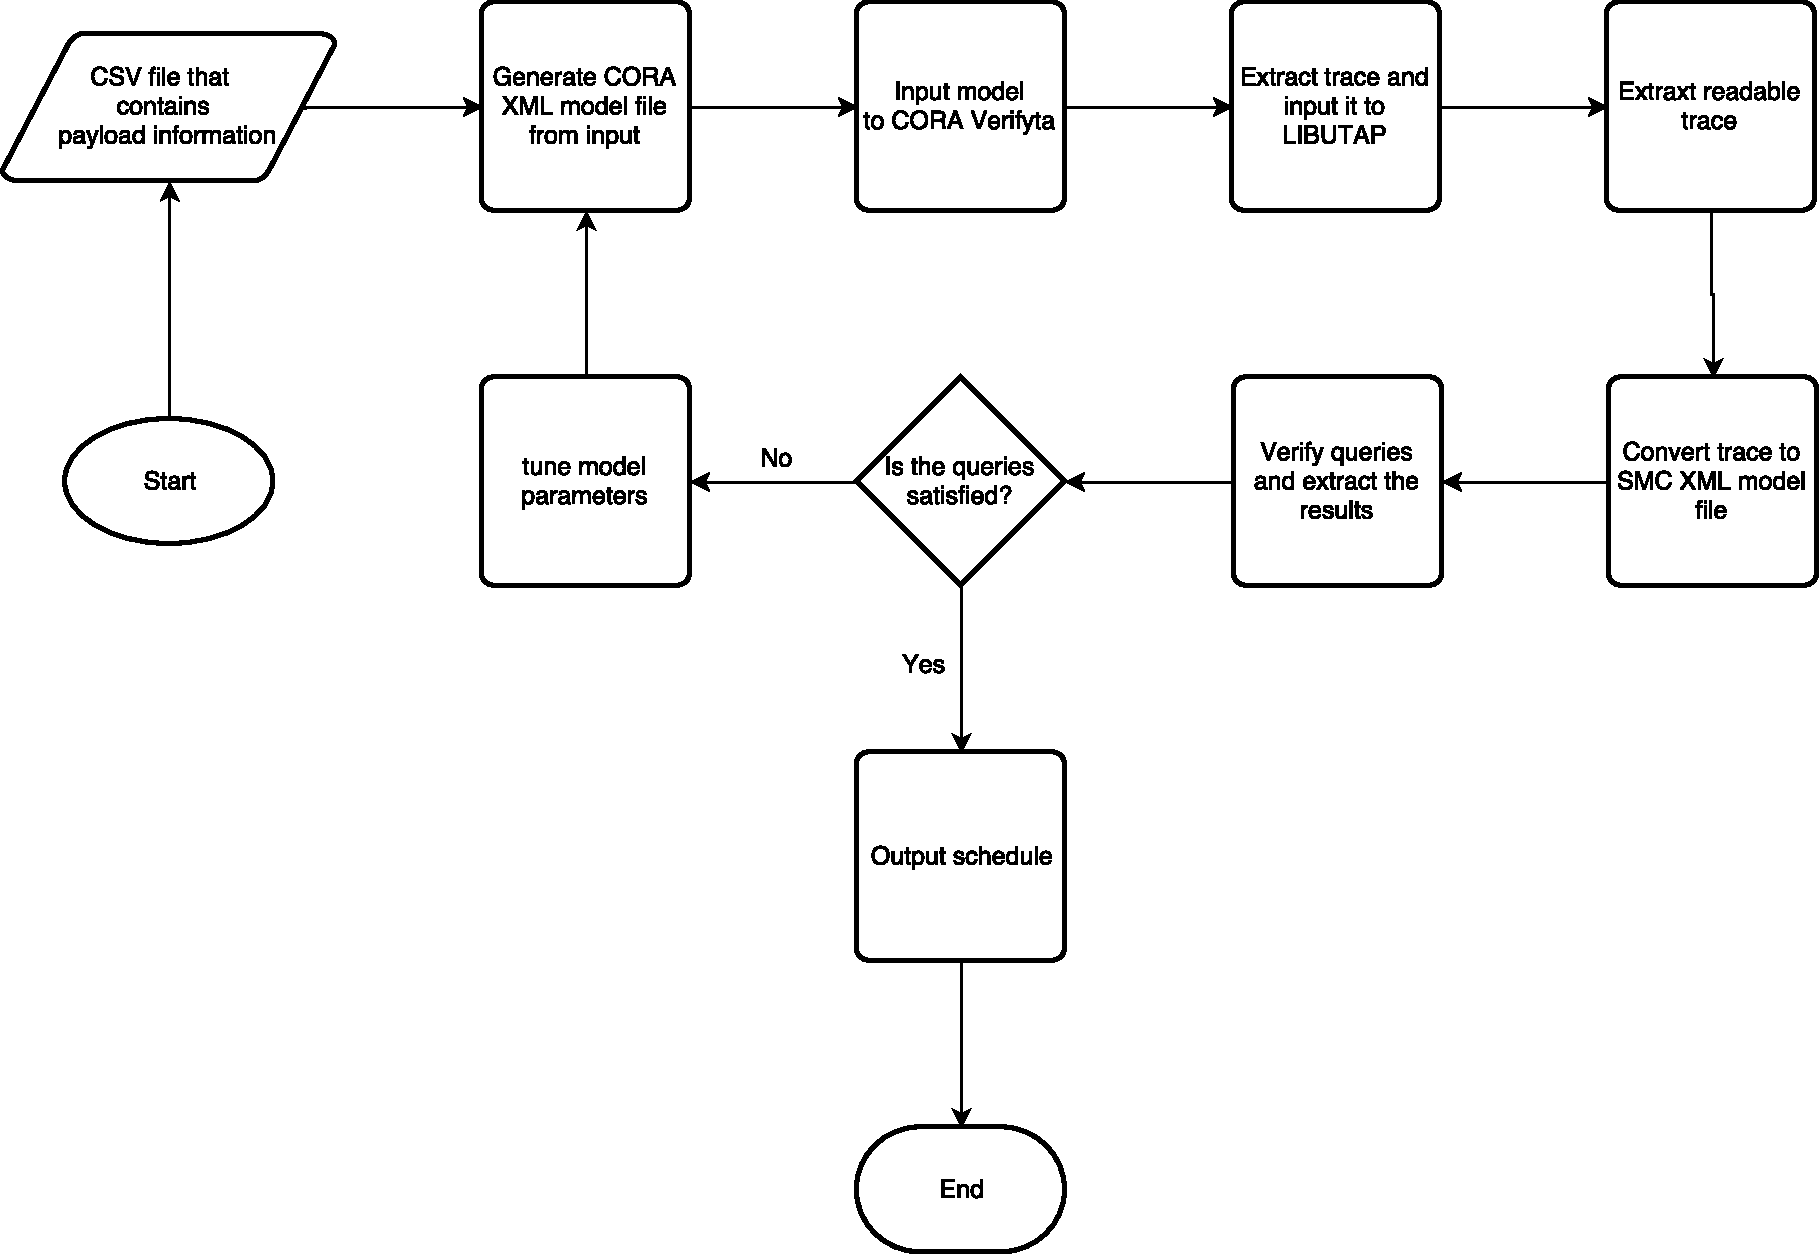
\includegraphics[width=\textwidth]{graphics/tool_chain.pdf}
	\label{fig:tool1}
	\caption{Flowchart that displays the workflow and use of tools}
\end{figure}

\paragraph{Location 1 - CSV file that contains payload information} 
Is the input file for the system. 
The usage of this file and its format is described in \cref{sec:read_input}.

\paragraph{Location 2 - Generate \gls{cora} XML models file from input} 
In this location we will read the CSV file or the tuned parameters from location 9. 
The input is used to generate two \gls{cora} models.
The values specified in the input file can be in a range to indicate variations or uncertainties in how much time, power, etc. a payload uses.
One model uses the worst case values and the other will use the interval. 

%\paragraph{Location 3 - Input model to CORA Verifyta} the Verfyta will generate a trace for each model.

\paragraph{Location 4 - Test worst case model} 
Run the queries on the worst case model.

\paragraph{Location 5 - Is the worst case possible?} 
If we were unable to produce a trace for the worst case, we will not be able to guarantee that any of the schedules we produce will stay within the specified parameters. 
We will as a result thereof go to location 6, the fail state.

\paragraph{Location 7 - Extract trace from the \gls{cora} model and it to \acrshort{lbtp}} 
In this location we will extract a trace from the \gls{cora} model and use it as input for the tracer function in \acrshort{lbtp}. 
The tracer function will transform the output into a readable trace which can be used later on.

%\paragraph{Location 9 - Convert trace to \gls{smc} xm model file} in this location we will read the trace and produce the \gls{smc} model that will be used in the next location.

\paragraph{Location 10 - Verify queries and extract the results} 
The \gls{smc} Verifyta will run the queries on the \gls{smc} model and output the results, see \cref{sec:smc}. 
These queries is made to validate and test the robustness of the trace.

\paragraph{Location 13 - Output schedule} 
If the queries are satisfied we will output the schedule, as this will indicate that the trace, or schedule, is correct.

\paragraph{Location 12 - Tune model parameters} 
If the queries were not satisfied, the schedule will be discarded and we will produce a new one. 
In order to produce a new schedule, we will provide \gls{cora} with a new set of parameters based on those from the CSV file. 
These parameters will be loyal to those specified in the CSV file, but their ranges will be shortened in order to provoke new choices in the schedule. 
This will change the workflow as we are not interested in verifying the worst case model any more, as the previous worst case is still true to this version of the parameters. 
We will therefore skip location 4, 5, and 6 and will go directly yo location 7.


\section{Schedule} \label{sec:schedule}
In order to produce a schedule we will first have to define what is considered a viable schedule. Different considerations goes into this, most impotently what is the requirements for a reliable schedule? The produced schedule should be correct and validated according to the specifications given as input.

First we will discuss what type of real-time the satellite is considered to be. It may be considered soft real-time, which means that if some deadlines fails it is not mission critical, it should however not be a common occurrence. In favour of the system being hard real-time is that the satellite can only perform some payloads within certain windows of time, such as communicating with earth, and must at that point be available to receive new schedules. \textit{As there are both soft- and hard real-time aspects to the satellite mission, it will be considered weakly hard real-time. This means that some deadlines must be upheld, where as others are not of the same level of importance.}

The schedule will need to be robust, meaning being capable of handling errors, such as; the satellite will sometimes have to restart at unforeseen times, or maybe the moon blocks the sun and the battery would therefore not recharge as much as expected. This may cause the satellite to fall behind schedule and would in some way need to compensate for this.
The battery level will have to be considered at all times, when producing and validating the schedule, and may never fall below a specified level, as it results in the satellite entering a safe mode where only the most necessary processes are allowed.
Therefore the schedule must accommodate this in a way such that there are no risk of the power level ever falling below the specified level.

A schedule is considered viable if it upholds the following criteria
\begin{enumerate}
	\item Battery level must at all times be above a certain level
	\item Schedule must give instructions from start to end
	\item Schedule must be optimal in regards to profit, while upholding other requirements such as battery level
\end{enumerate}
The first requirement will be referred to as a threshold and must be specified by the user during configuration.\\
The second requirement is there to allow the user to inspect every single step of the schedule, from start to end.\\ 
The goal of the third requirement is make sure that the nanosatellite are doing something worthwhile. This is why we introduce the profit aspect which should reflect actions that provides value, such as collecting data.

% Weakly hard
% http://ieeexplore.ieee.org/stamp/stamp.jsp?arnumber=919277
% Reasoning: We can do a lot of things whenever, but have to send data in surtain windows, and must receive new schedules at some point
\section{Reading the Input} \label{sec:read_input}
In order to model the payloads, battery, and schedule properties, we will need some information from the user.
The payloads are described through an input file where the dimensions represents the variables which will be used when producing the schedule.
The other properties related to the nanosatellite, is described in a configuration file.\\
We have filled out both files to provide examples of how to use them. It is expected that the user sets all of the variables in order to represent their system.

\subsection{Payload Specification} \label{subsec:csv}
The payloads are defined by eight variables and are defined in a CSV file. An example of this file with five payloads can be seen in \cref{lst:csv}. 
These payloads are based on those from the GomX-3 nanosatellite\cite{gomx3}.\\
The eight variables are Name, Time, Energy, Profit, Deadline, Dependencies, Window, and MaxRuns.\\
\textbf{Name} should indicate what the payload represents. When modelled, a payloads name will be translated into a number in range 0 to N-1 where N is the amount of payloads. The numeric name will also be used when a payload is referenced in the produced schedule.\\
\textbf{Time} specifies how much time, in minutes, it will take to complete the payload. It is defined by a range in order to allow for uncertainty in regards to the timing of the payloads. It is valid to specify a number that is higher than the orbit duration, but a time may not be below 0.\\
\textbf{Energy} specifies how high a load, in mAh, the payload applies on the battery every minute it is being executed.\\
\textbf{Profit} is expressed within a range from 1 to 5, which signifies how valuable or profitable it is to complete a payload. 1 being the least profitable and 5 being the most. In the example from below, L1 and L2 represents the use of the L-Band transmitter that the GomX-3 nanosatellite use to communicate with other satellites, which allows it to collect valuable data. Which is why it has been given a profit of 5 as it is the most profitable payload. The first payload Slew represents the action of slewing the nanosatellite. This does not directly generate any profit for the nanosatellite as no data is gathered.\\
\textbf{Deadline} is a positive integer and is used to cancel payloads which are delayed too much. The minimum value for the deadline is that of the maximum execution time and the maximum is undefined. The scheduler may chose to wait before executing a payload and we can therefore risk that it is no longer relevant to execute the next payload in the queue.
The decision for whether or not to cancel a payload in regards to its deadline goes as follows: \textit{if the time we have spent waiting for the next payload to start plus the time it takes to complete the payload exceeds the deadline; then cancel}. We want to make sure that only payloads that are guaranteed to finish within their deadline start\\
\textbf{Dependencies} contains a list of other payloads which the current payload is waiting for to be completed. A payload may only be executed if all payloads expressed in its dependencies have previously been activated. The user may specify a dependency of multiple executions of another tasks. In the example, X is dependant on L1 and L2 to be completed twice, before it may self be executed.\\
Some payloads can only be executed in a certain time \textbf{Window}, such as when they are above the communication station on Earth.
This is why we have added the variable which restricts when payloads can be executed as it may only happen within the window. The window is specified by a range with the minimum value of 0 and the maximum is equal to the the orbit time. If a payload does not have an associated window it will be allowed to run at any given time, given its dependencies are fulfilled.\\
In addition we have added the concept of \textbf{MaxRuns} which indicates the amount of times each payload can be executed in a payload cycle. A payload cycle is completed when all of the payloads have been executed as many times as described by their MaxRuns value. Whenever a payload has been completed an associated counter, that belongs to the payload, is incremented. When all payloads have reached the MaxRuns value, their individual counter is set to $0$ and a new payload cycle begins. All dependencies are also being reset when a new cycle begins, which means that payloads will need to wait for their dependencies to be completed again. This is done to avoid executing the same payload for the duration of the schedule as soon as its dependencies are fulfilled. MaxRuns is a constant and all payloads must be set to $1$ or higher.
\begin{figure}[H]
\begin{lstlisting}[caption={Example of how five payloads can be defined}, label=lst:csv, language=text]
Name,	Time,	Energy,	Profit,	Deadline,	Dependencies,Window,MaxRuns
Slew,	2-5,	10,		1,		85,			-1,			-1,		3
L1,		90-90,	20,		5,		120,		-1,			-1,		3
L2,		90-90,	20,		5,		120,		-1,			-1,		2
X,		15-15,	10,		3,		30,			0 2 2 0 0,	45-60,	2
UHF,	15-15,	15,		1,		45,			0 0 0 1 0,	20-65,	1
\end{lstlisting}
\end{figure}

\subsection{Configuration Specification} \label{subsec:init}
The nanosatellite and its battery is specified by a configuration which consists of a list of variables and constants. The configuration is read from an INI file which we have provided an example of below in \cref{lst:ini}.
The configuration is divided into three sections System, CORA, and SMC.\\
The System specific variables describes the nanosatellite and the time constraints.
The variables are:
\begin{itemize}
	\item schedule\_length
	\item orbit\_time
	\item battery\_capacity
	\item idle\_cost
	\item safe\_threshold
	\item soc
	\item rec\_rate
\end{itemize}
The \textbf{schedule\_length} defines how long the produced schedule should be, in minutes. 
\textbf{orbit\_time} defines how long it takes to complete one orbit, in minutes. 
The \textbf{battery\_capacity} is an constant that defines the maximum capacity of the battery. We do not expect that the user defines every single operation that the nanosatellite is capable of performing, which is why we have made an abstraction by introducing the \textbf{idle\_cost} variable. 
\textbf{idle\_cost} is the load that is imposes on the battery at all times, even when the nanosatellite is idling, not currently executing any of the defined payloads.
This will allow us to disregard some of the payloads that the nanosatellite may perform as they can be grouped together as one single background process which is always being executed.
The user should only consider payloads which can be executed in parallel to the defined payloads and only chose those which energy and time cost are trivial.
Failing to do so may result in a non representative model of their nanosatellite and therefore a schedule where our guarantees may not be valid.\\
Based on the findings from Bisgaard et al. 2016\cite{gomx3} we have decided to include the \textbf{safe\_threshold} variable.
This variable is used to determine when the nanosatellite's \gls{soc} is too low to continue executing the schedule.
If the nanosatellite go below this threshold, it is in danger of depleting the battery, which means it will not be able to communicate with Earth for a period of time.
This will result in a huge loss of potential profit as we are no longer able to execute profitable payloads and should therefore be avoided.It is critical that the schedules we produce will never go below this threshold.\\
\textbf{rec\_rate}  defines the recharge rate such that the value is added to the battery's capacity every minute that the nanosatellite is in insolation.\\
We have three variables that are related to the \gls{smc} model where two of them is used in its battery model.\\
\begin{itemize}
	\item f\_rate
	\item ac\_width
	\item certainty
\end{itemize}
\textbf{f\_rate} is a rate that is specific to the battery model we have chosen, and it is used to simulate the recovery effect of batteries. The recovery effect will be described later in \myref{sec:kibam}, together with the \textbf{ac\_width} constant.
The constant \textbf{certainty} specifies how certain we require that \gls{smc} should be in its results. \gls{smc} is described in \myref{sec:smc}.
\begin{figure}[H]
\begin{lstlisting}[caption={Example of how the environment can be defined}, label=lst:ini, language=text]
[SYSTEM]
# System specific
# schedule length in minutes
schedule_length = 720
# orbit time in minutes
orbit_time = 90
# battery capacity in mAh
battery_capacity = 5400
# idle cost in mAh
idle_cost = 1
# safe mode threshold in percentage [0-100]
safe_threshold = 40
# The start SoC in mAh
soc = 4800

[CORA]
# Cora specific

[SMC]
# SMC specific
# Recharge rate
rec_rate = 4.2
# flow of available charge
f_rate = 0.0002324
# available width in relation to bound width
ac_width = 0.16667
# how certain should the system be in the results? Percentage [1-99]
certainty = 95
\end{lstlisting}
\end{figure}
At this point the CORA section does not contain any variables, the section is used as a placeholder for future versions of the system, as the model could be expanded to include variables specific to \gls{cora}.

Now that payloads and nanosatellite is specified, we are able to start modelling the system.

\section{UPPAAL} \label{sec:uppaal}
We have chosen to use \acrlong{cora}\cite{cs_cora}\cite{cora_tutorial} and \acrlong{smc}\cite{smc_home}\cite{cs_smc} for producing and verifying the schedule. We will describe the common charismatics for both versions and then introduce them before their respective models are presented.

Common for all versions of UPPAAL, is that; it has global decelerations and templates. 
An example template can be seen in \cref{fig:uppaal_eksample}.
One model may have several templates, each with its own local decelerations. The template itself consists of one to many locations and edges that connects the locations.\\
One location in each template must be initial in order for UPPAAL to determine the starting state. In addition a location can be urgent, meaning time is not allowed to pass while the location is active, or committed which is a stronger expression than urgent. Committed indicates that activating an outgoing transition is of priority. If any committed location in the model is part of the current state, at least one transition from a committed location must be part of the next transition.
Edges may be decorated with; selects, guards, synchronizations, and updates. 
Selects are used for introducing new temporary variables, and are coloured yellow.
Guards are used to ensure that an edge is not activated prematurely, and are coloured green.
Synchronizations are used for activating multiple edges across templates simultaneously, and are coloured light blue. If an exclamation mark is used, it indicates that it is calling a synchronisation, whereas a question mark is receiving one.
Finally updates are used to change variable values, and to call functions written in declarations, and are coloured dark blue.\\
Locations can be given a name and an invariant. An invariant must always be evaluated to true e.g. if a location have the invariant $time <= 5$, at time five there will be a chance of state. Invariants are coloured pink.\\
Also common for the versions of UPPAAL, is that queries can be written in order to ensure sustain properties are upheld, such as; is some location reachable, and will time ever exceed some amount.

\begin{figure}[h]
   \centering
   \begin{tikzpicture}
   %Locations
   \node [init, label = {
           [align=left]above:
           \textcolor{name}{location A}
       }] (l0) {$\cup$};
   \node [location] (l1) [right of=l0, xshift=30mm, label={
        [align=right]above:
       \textcolor{name}{Location B}\\
       \textcolor{invariant}{x <= myLimit}}
   ] {};
   \node [location] (l2) [right of=l1, xshift=40mm, label={
       [align=right]above:
       \textcolor{name}{location C}
   }] {};

   \path[->,black, thick] (l0) edge node [midway, below ][align=center]{\textcolor{update}{mayRun()}} (l1);
   \path[->,black, thick] (l1) edge node [midway, below][align=center]{
   \textcolor{select}{a: int[0,N-1]}\\
           \textcolor{guard}{everythingIsGood() == true}\\
           \textcolor{sync}{ready!}\\
           \textcolor{update}{changeValue(), myVar = a}} (l2);
   \end{tikzpicture}
   \caption{Example template}
   \label{fig:uppaal_eksample}
\end{figure}

\section{UPPAAL CORA}\label{sec:upp_cora}
UPPAAL \acrfull{cora} is a branch of UPPAAL, that uses linearly priced timed automata to find optimal paths satisfying certain goals, based on lowest accumulated cost\cite{cs_cora}. Cost is a variable that can be only be interacted with through locations, where it is possible to define the incremental rate with which it will grow, with the passing of time. 
Which means that if a location's rate is 5, and two time units passes, the cost will grow by 10. It allows \gls{cora} to prune traces, if two traces reach the same location where all variables for each of the traces are identical expect for the cost variable, the trace with the lowest cost will be kept to preserve memory. 
Due to the underlying structure of \gls{cora} it is only possible to do reachability checks, and does not allow for liveness or deadlocks checks.
Only best first search is supported when we are searching for the best trace. Lastly \gls{cora} cannot guarantee termination unless the modelled system is acyclic and clocks are bound by invariants.

\Gls{cora} have been used in a range of problems regarding scheduling problems, the most related case for our problem is GomX-3 case, where they used \gls{cora} to generate a battery aware schedule for CubeSat satellite. Their solution takes a set of parameters to generate fractions of the entire schedules and, when all parts of the schedule is generated, they are assembled by appending them in a chronological order. Lastly, the acummulated schedule is tested with an external \gls{kibam} battery model.

\Gls{cora} introduced the concept of cost, which as mentioned is accumulated over time. An example of how such a model may look can be seed in \cref{fig:cora_eks}.

\begin{figure}[H]
	\centering
	\begin{tikzpicture}
	%Locations
	\node [init] (l0) [label={
		[align=left]above:
		\textcolor{name}{A}
	}, label={
		[align=left]left:
		\textcolor{invariant}{cost '== 1}\\
		\textcolor{invariant}{\&\& time <= 5}
	}] {};
	\node [location] (l1) [right of=l0, xshift=20mm, yshift=20mm, label={
		[align=left]above:
		\textcolor{name}{B1}
	}, label={
		[align=left]below:
		\textcolor{invariant}{cost '== 1}\\
		\textcolor{invariant}{\&\& time <= 5}
	}] {};
	\node [location] (l2) [right of=l0, xshift=20mm, yshift=-20mm, label={
		[align=left]above:
		\textcolor{name}{B2}
	}, label={
		[align=left]below:
		\textcolor{invariant}{cost '== 1}\\
		\textcolor{invariant}{\&\& time <= 5}
	}] {};
	\node [location] (l3) [right of=l2, xshift=20mm, yshift=20mm, label={
		[align=left]above:
		\textcolor{name}{C}
	}, label={
		[align=left]right:
		\textcolor{invariant}{cost '== 1}\\
		\textcolor{invariant}{\&\& time <= 5}
	}] {};
	%Edges
	\path[->,black, thick] (l0) edge node [midway, left][align=left]{
			\textcolor{guard}{time >= 3}} (l1);
	\path[->,black, thick] (l0) edge node [midway, left][align=left]{
			\textcolor{guard}{time >= 3}} (l2);
	\path[->,black, thick] (l1) edge node [midway, right][align=left]{
			\textcolor{guard}{time >= 10}} (l3);
	\path[->,black, thick] (l2) edge node [midway, right][align=left]{
			\textcolor{guard}{time >= 7}} (l3);
	\end{tikzpicture}
	\caption{Simple model made in \gls{cora}, which displays an increase in cost over time}
	\label{fig:cora_eks}
\end{figure}

In \cref{fig:cora_eks} we see a \gls{cora} model with four locations and four edges connecting them. On three of the location there is an invariant bound to the clock "\uppVar{time}" and an associated cost rate. While in the initial location "\uppLoc{A}" the cost rate is one meaning that for every unit of time spend in this \uppLoc{A} the cost will increase by one, it will stay in \uppLoc{A} for three to five units of time before moving on to the next location.\\
After this is where the model gets interesting, there are at this point two possible transitions, it may move to either "\uppLoc{B1}" or "\uppLoc{B2}". In \uppLoc{B1} the cost will increase with a rate of 3 per unit of time and will stay there until time reaches ten. Alternatively it may transition to \uppLoc{B2} where the cost rate is four and will stay there until time is between seven and ten. After visiting one of these locations it will reach the final state "\uppLoc{C}". \\
In UPPAAL we can then run the query seen in \cref{eq:cora_get_c}, a simple query asking if location \uppLoc{C} is reachable, however in \gls{cora} the settings for diagnostic trace allows us to get the best trace, meaning the one with the smallest cost.
\begin{align}
E<> Template.C
\label{eq:cora_get_c}
\end{align}
This is beneficial as the optimal route may not always be what seems to be the obvious one. We see in \cref{fig:cora_eks} that \uppLoc{B1} only have a cost of three per tic whereas \uppLoc{B2} have a cost of four per tic, however it is required to stay in \uppLoc{B1} for a longer period of time, actually causing the bottom route to become cheaper.
The model in \cref{fig:cora_eks} is of course a simple one,

%This can be advantageous for modelling systems such as satellites where energy is an important and limited resource which can be represented by the cost. After running a query it is possible to extract a trace, which can be used to represent the generated schedule.

%http://people.cs.aau.dk/~adavid/cora/download.html#download


%optimal sceduling and planning.
%state-space exploration -> promising and cheap visited first -> prune parts of search tree not improving solution.
%symbolic data structure -> symbolic state-space representation with cost information -> optimal or near-optimal solutions

%S2,3: problem of cost-optimal reachability -> symbolic branch-and-bound solving this problem.
% clocks are non-negative real values, can be reset and grow at a fixed rate.

%S5: PTA-related optimization problems -> future support


\section{Battery Models} \label{sec:kibam}
Part of the proposed solution is to ensure that battery level are maintain at an expectable level, in order to do this we need some way of modelling a battery, this section will go over three different battery models to determine what drawbacks there may be when using certain battery models. An important factor to consider when examining the battery models is the recovery effect, which can have large impact on the expected lifetime\cite{battery_model}. Recovery effect happen after a battery has been discharged for a period of time, the amount of current applied to the battery effects the recovery effect along with the battery capacity. The performance of the different models will be compared to the actual measured of a lithium-ion battery, measured are taken from \cite{battery_lifetime_analysis}, unfortunatly we are unable to obtain the specification for the lithium battery used in the paper as they are not listed in the paper. The measures for the different battery models is taken from \cite{battery_model} which also uses the same battery specification as the other paper they claim.

The Ideal model is very simplistic due to it only having two variables to determine the batteries lifetime(L), capacity(C) and load current(I). Capacity relates to the batteries amount of amp-hours, and load current is the constant discharge on the battery in amps. The formal for this is shown in \cref{eq:bm}.

\begin{equation}\label{eq:bm}
L=C/I
\end{equation}

Performance of the Ideal model can be seen in \cref{table:t-Ideal}. The table is divided into two parts, constant load and variable load, the column ``Meas, min'' show the actual measured readings of the lithium-ion battery under different loads. To the right the Ideal estimation are shown. In general the Ideal model overestimate the expected lifetime in all cases, shown in T1 the deviation from the actual measures differs by 28.58\%, a trend seems to appear in that lower amps often results in better predictions from the Ideal model with constant loads. Only T5 and T6 dose not apply to this, because T5 have a better prediction then T6 even though T5 has a higher load. During variable loads all cases overestimate by a substantial amount, the closest approximation is C5 during variable loads with a 18.5\% overestimation. The data shows that the Ideal model does a poor job of estimating the actual lifetime of a battery, which is properly because the Ideal model assumes linear effect for lifetime estimation. Additionally for variables loads the Ideal model does not consider recovery effect of the battery which further deviate results from the measured values. 

% Please add the following required packages to your document preamble:
% \usepackage[table,xcdraw]{xcolor}
% If you use beamer only pass "xcolor=table" option, i.e. \documentclass[xcolor=table]{beamer}
\begin{table}[H]
	\centering
	\scalebox{0.8}{
	\begin{tabular}{|llllll|lllll|}
		\hline
		\multicolumn{6}{|c|}{Constant load} & \multicolumn{5}{c|}{Variable load} \\ \hline
		\rowcolor[HTML]{EFEFEF} 
		\multicolumn{1}{|l|}{\cellcolor[HTML]{EFEFEF}Test} & \multicolumn{1}{l|}{\cellcolor[HTML]{EFEFEF}I, amps} & \multicolumn{1}{l|}{\cellcolor[HTML]{EFEFEF}Meas, min} & \multicolumn{1}{l|}{\cellcolor[HTML]{EFEFEF}Ideal, min} & \multicolumn{1}{l|}{\cellcolor[HTML]{EFEFEF}$\Delta$T} & \%$\Delta$ & \multicolumn{1}{l|}{\cellcolor[HTML]{EFEFEF}Test} & \multicolumn{1}{l|}{\cellcolor[HTML]{EFEFEF}Meas, min} & \multicolumn{1}{l|}{\cellcolor[HTML]{EFEFEF}Ideal, min} & \multicolumn{1}{l|}{\cellcolor[HTML]{EFEFEF}$\Delta$C} & \%$\Delta$ \\ \hline
		T1 & 222.7 & 141.0 & 181.3 & 40.3 & 28.58\% & C1 & 54.5 & 70.8 & 16.3 & 29.91\% \\ \hline
		\rowcolor[HTML]{EFEFEF} 
		T2 & 204.5 & 156.6 & 197.4 & 40.8 & 26.05\% & C2 & 73.3 & 91.9 & 18.6 & 25.38\% \\ \hline
		T3 & 108.3 & 307.8 & 372.8 & 65 & 21.12\% & C3 & 88.3 & 108.5 & 20.2 & 22.88\% \\ \hline
		\rowcolor[HTML]{EFEFEF} 
		T4 & 107.5 & 312.0 & 375.6 & 63.6 & 20.38\% & C4 & 136.0 & 163.0 & 27 & 19.85\% \\ \hline
		T5 & 94.9 & 358.2 & 425.4 & 67.2 & 18.76\% & C5 & 182.7 & 216.5 & 33.8 & 18.50\% \\ \hline
		\rowcolor[HTML]{EFEFEF} 
		T6 & 84.3 & 397.2 & 478.9 & 81.7 & 20.57\% & C6 & 59.0 & 74.7 & 15.7 & 26.61\% \\ \hline
		T7 & 75.5 & 448.2 & 534.8 & 86.6 & 19.32\% & C7 & 51.1 & 66.9 & 15.8 & 30.92\% \\ \hline
		\rowcolor[HTML]{EFEFEF} 
		T8 & 28.0 & 1248 & 1442 & 194 & 15.54\% & C8 & 55.0 & 70.8 & 15.8 & 28.73\% \\ \hline
		T9 & 19.5 & 1818 & 2071 & 253 & 13.92\% & C9 & 54.9 & 70.8 & 15.9 & 28.96\% \\ \hline
		\rowcolor[HTML]{EFEFEF} 
		T10 & 3.0 & 12690 & 13458 & 768 & 6.05\% & C10 & 142.7 & 171.3 & 28.6 & 20.04\% \\ \hline
	\end{tabular}}
	\caption{Comparison of actual measure and measures from Ideal model. Specification for the variable loads can be found in \cref{table:variable_loads_list}
	}
	\label{table:t-Ideal}
\end{table}

Peukert Model introduces a few new variables in comparison to the Ideal model, like the previous we still want to estimate the expected lifetime, but to better represent the battery a non-linear model is needed. Peukert fixes this by changing the formula to what is seen in \cref{eq:pm}. 

\begin{equation}\label{eq:pm}
L=(\frac{C}{I^k})
\end{equation}
\begin{itemize}
	\item L - lifetime in hours
	\item C - capacity in AH
	\item I - load current in amps
	\item k - Peukert Exponent
\end{itemize}

Unlike the previous model these parameter not as concrete. Acording to \cite{battery_modeling} C should be close to the value of the battery capacity and k should be between 1.2 and 1.7 to give the best results. This should be noted that this is only for constant loads. as it best illustrate how Peukert model functions\cite{battery_modeling}. k can sometimes be provided by the manufactors, since it can be hard to determine the exact value of k without actual testing a battery

\cref{table:t-Peukert} showcases the estimations using Peukert. In most cases Peukert overestimate except for one instance in test T10, it underestimate with 3.17\%. It seems to become more accurate the smaller the amps are, with the outlines, T5 and T6 Similarly to \cref{table:t-Ideal}. One thing to notices is that for variable loads it still has a high mismatch compared to measured values, this is due to Peukerts model not taken recovery effect into account. But overall Peukert performance better than the Ideal model.

\begin{table}[H]
	\centering
	\scalebox{0.8}{
	\begin{tabular}{|llllll|lllll|}
\hline
\multicolumn{6}{|c|}{Constant load} & \multicolumn{5}{c|}{Variable load} \\ \hline
\rowcolor[HTML]{EFEFEF} 
\multicolumn{1}{|l|}{\cellcolor[HTML]{EFEFEF}Test} & \multicolumn{1}{l|}{\cellcolor[HTML]{EFEFEF}I, amps} & \multicolumn{1}{l|}{\cellcolor[HTML]{EFEFEF}Meas, min} & \multicolumn{1}{l|}{\cellcolor[HTML]{EFEFEF}Peukert, min} & \multicolumn{1}{l|}{\cellcolor[HTML]{EFEFEF}$\Delta$T} & \%$\Delta$ & \multicolumn{1}{l|}{\cellcolor[HTML]{EFEFEF}Test} & \multicolumn{1}{l|}{\cellcolor[HTML]{EFEFEF}Meas, min} & \multicolumn{1}{l|}{\cellcolor[HTML]{EFEFEF}Peukert, min} & \multicolumn{1}{l|}{\cellcolor[HTML]{EFEFEF}$\Delta$C} & \%$\Delta$ \\ \hline
T1 & 222.7 & 141.0 & 154.5 & 13.5 & 9.57\% & C1 & 54.5 & 60.5 & 6 & 11.01\% \\ \hline
\rowcolor[HTML]{EFEFEF} 
T2 & 204.5 & 156.6 & 168.4 & 11.8 & 7.54\% & C2 & 73.3 & 79.1 & 5.8 & 7.91\% \\ \hline
T3 & 108.3 & 307.8 & 321.3 & 13.5 & 4.39\% & C3 & 88.3 & 93.8 & 5.5 & 6.23\% \\ \hline
\rowcolor[HTML]{EFEFEF} 
T4 & 107.5 & 312.0 & 323.7 & 11.7 & 3.75\% & C4 & 136.0 & 142.5 & 6.5 & 4.78\% \\ \hline
T5 & 94.9 & 358.2 & 367.5 & 9.3 & 2.60\% & C5 & 182.7 & 190.2 & 7.5 & 4.11\% \\ \hline
\rowcolor[HTML]{EFEFEF} 
T6 & 84.3 & 397.2 & 414.4 & 17.2 & 4.33\% & C6 & 59.0 & 64.4 & 5.4 & 9.15\% \\ \hline
T7 & 75.5 & 448.2 & 463.6 & 15.4 & 3.44\% & C7 & 51.1 & 56.5 & 5.4 & 10.57\% \\ \hline
\rowcolor[HTML]{EFEFEF} 
T8 & 28.0 & 1248 & 1270 & 22 & 1.76\% & C8 & 55.0 & 60.5 & 5.5 & 10.00\% \\ \hline
T9 & 19.5 & 1818 & 1835 & 17 & 0.94\% & C9 & 54.9 & 60.5 & 5.6 & 10.20\% \\ \hline
\rowcolor[HTML]{EFEFEF} 
T10 & 3.0 & 12690 & 12288 & -402 & -3.17\% & C10 & 142.7 & 148.8 & 6.1 & 4.27\% \\ \hline
\end{tabular}}
	\caption{Comparison of actual measure and measures from Peukert model. Specification for the variable loads can be found in \cref{variable_loads_list}
	}
	\label{table:t-Peukert}
\end{table}

\gls{kibam} uses two wells as an abstract concept to represent a battery. It consist of an available charge and a bound charge as shown in \cref{fig:kibam_wells}, c determines the ratio of the two wells based on the total capacity. Current can only be drawn from the available charge, when the available charges height $h_2$ is lower then bound charge height $h_1$, charge start to flow from bound charge to available charge until both wells are at equal height. The rate of this flow is determined by the value k, this simulate the recovery effect of the battery like previous models was not able to capture. To calculate $y{1}$ and $y{2}$ can be seen in \cref{eq:y1} and\cref{eq:y2} along with a short description of the variables used in these equations.

\begin{figure}[H]
	\center
	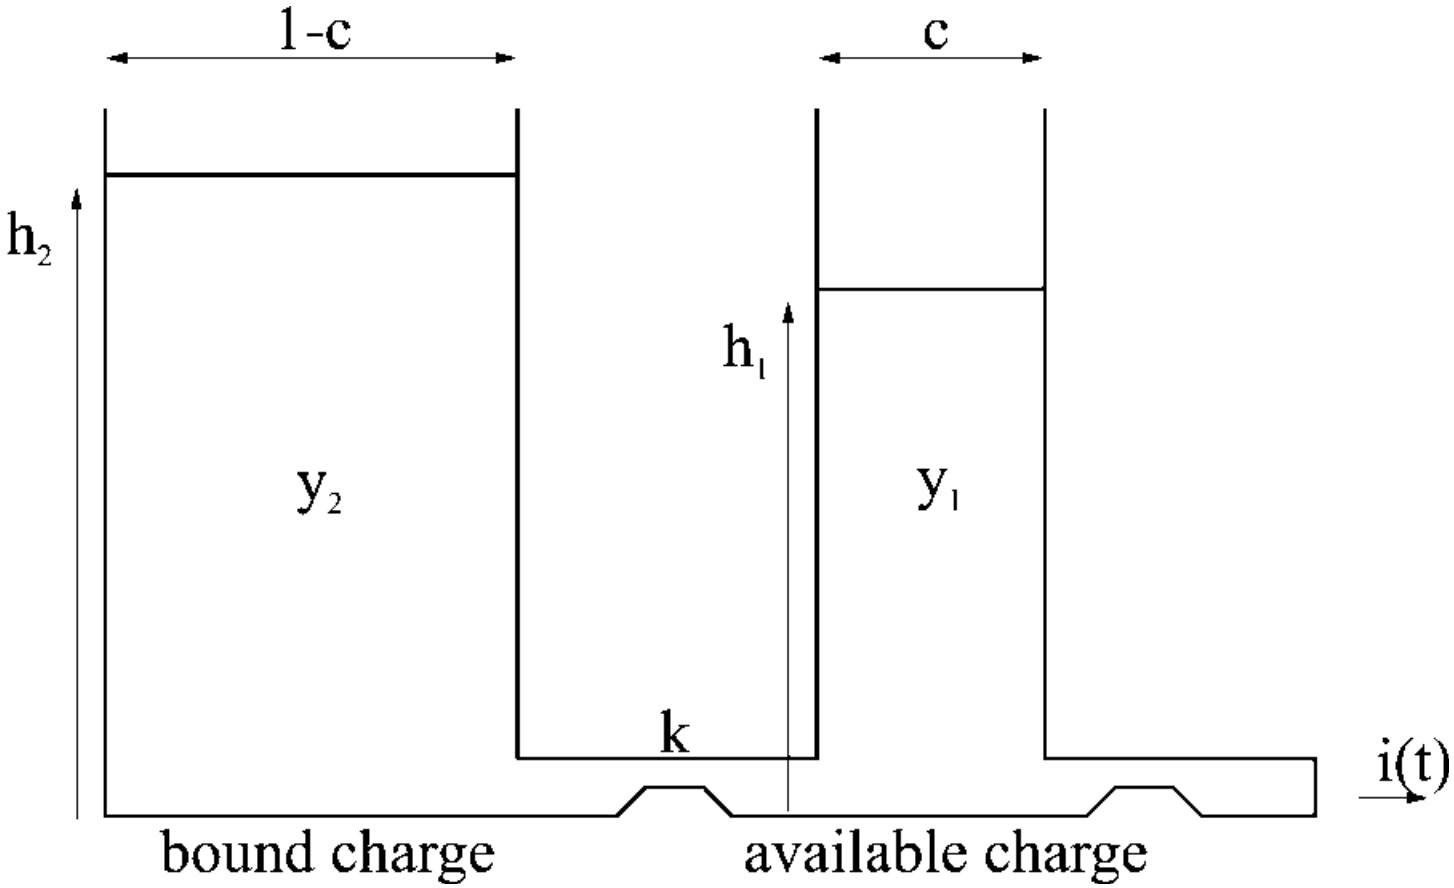
\includegraphics[width=\textwidth/2]{graphics/kibam.jpg}
	\caption{Displays the two wells of \gls{kibam}}
	\label{fig:kibam_wells}
\end{figure}

\begin{equation}\label{eq:y1}
y_1(t) = cCe^{-k't}+\frac{(y_0k'c-I)(1-e^{-k't})}{k'}-\frac{Ic(k't-1+e^{-k't})}{k'}
\end{equation}

\begin{equation}\label{eq:y2}
y_2(t) = (1-c)Ce^{-k't}+y_0(1-c)(1-e^{-k't})-\frac{I(1-c)(k't-1+e^{-k't})}{k'}
\end{equation}

C is capacity in Ah, e is Euler's number, k' is $k/c(1-c)$, k is a constant, t is time in hours, c is the ratio between available and bound charge, and I is the load current applied on the battery.

Performance of \gls{kibam} can be seen in \cref{table:t-KiBaM}. Under constant load the results vary, and he only indicating is that an amps above 110 and below 20 seems to give better results. Interesting for variable loads is that all of the predictions from \gls{kibam} underestimate compared to the measured values, some are fairly high though, like in case C7 it underestimate by 40.31\%.

\begin{table}[]
	\centering
	\scalebox{0.8}{
	\begin{tabular}{|l|lllll|llll|l|}
\hline
\multicolumn{6}{|c|}{Constant load} & \multicolumn{5}{c|}{Variable load} \\ \hline
\rowcolor[HTML]{EFEFEF} 
Test & \multicolumn{1}{l|}{\cellcolor[HTML]{EFEFEF}I, amps} & \multicolumn{1}{l|}{\cellcolor[HTML]{EFEFEF}Meas, min} & \multicolumn{1}{l|}{\cellcolor[HTML]{EFEFEF}KiBaM, min} & \multicolumn{1}{l|}{\cellcolor[HTML]{EFEFEF}$\Delta$T} & \%$\Delta$ & \multicolumn{1}{l|}{\cellcolor[HTML]{EFEFEF}Test} & \multicolumn{1}{l|}{\cellcolor[HTML]{EFEFEF}Meas, min} & \multicolumn{1}{l|}{\cellcolor[HTML]{EFEFEF}KiBaM, min} & $\Delta$T & \%$\Delta$ \\ \hline
T1 & 222.7 & 141.0 & 139.9 & -1.1 & -0.78\% & C1 & 54.5 & 36.3 & -18.2 & -33.39\% \\ \hline
\rowcolor[HTML]{EFEFEF} 
T2 & 204.5 & 156.6 & 156 & -0.6 & -0.38\% & C2 & 73.3 & 55.7 & -17.6 & -24.01\% \\ \hline
T3 & 108.3 & 307.8 & 331.4 & 23.6 & 7.67\% & C3 & 88.3 & 71.4 & -16.9 & -19.14\% \\ \hline
\rowcolor[HTML]{EFEFEF} 
T4 & 107.5 & 312.0 & 334.1 & 22.1 & 7.08\% & C4 & 136.0 & 123.6 & -12.4 & -9.12\% \\ \hline
T5 & 94.9 & 358.2 & 384 & 25.8 & 7.20\% & C5 & 182.7 & 175.7 & -7 & -3.83\% \\ \hline
\rowcolor[HTML]{EFEFEF} 
T6 & 84.3 & 397.2 & 437.5 & 40.3 & 10.15\% & C6 & 59.0 & 41.1 & -17.9 & -30.34\% \\ \hline
T7 & 75.5 & 448.2 & 493.3 & 45.1 & 10.06\% & C7 & 51.1 & 30.5 & -20.6 & -40.31\% \\ \hline
\rowcolor[HTML]{EFEFEF} 
T8 & 28.0 & 1248 & 1401 & 153 & 12.26\% & C8 & 55.0 & 38.1 & -16.9 & -30.73\% \\ \hline
T9 & 19.5 & 1818 & 2029 & 211 & 11.61\% & C9 & 54.9 & 34.8 & -20.1 & -36.61\% \\ \hline
\rowcolor[HTML]{EFEFEF} 
T10 & 3.0 & 12690 & 13417 & 727 & 5.73\% & C10 & 142.7 & 131.7 & -11 & -7.71\% \\ \hline
\end{tabular}}
	\caption{Comparison of actual measure and measures from \gls{kibam}. Specification for the variable loads can be found in \cref{variable_loads_list}
	}
	\label{table:t-KiBaM}
\end{table}

Looking at all the results for the three battery models, it show that Peukerts model give overall better estimation for variable loads then Ideal and \gls{kibam}. But the advantage of using \gls{kibam} over Peukerts model under variable load is that \gls{kibam} seems always underestimate, which is good for our case, that ensure that we will never run into a case where the prediction cause the actual system to run out of energy. The Ideal is inferior to Peukerts and \gls{kibam} in almost all predictions, a summarize of the three different battery models can be found below.
\begin{itemize}
	\item Ideal model - linear representation of the battery with no support of recovery effect
	\item Peukert model - non-linear representation of the battery with no support of recovery effect
	\item \gls{kibam} - abstract representation of the battery with support of recovery effect
\end{itemize}
Since CORA can not use \gls{kibam} or Peukert model because \gls{cora} only support price with a linear rate and only natural numbers. The Ideal model will have to suffice.

\section{Cora Model} \label{sec:cora}
The \gls{cora} model takes a set of tasks with some rules and constrains in order to generate a schedule that upholds the specifications. These are fed to the model from the csv file via our own translator.



\subsection*{Task}
\begin{figure}
	\centering
	\begin{tikzpicture}
	%Locations
	\node [init] (l0) {$\cup$};
	\node [location] (l1) [right of=l0, xshift=40mm] {$\cup$};
	\node [location] (l2) [right of=l1, xshift=40mm, label={
		[align=left]right:
		\textcolor{name}{ready}
	}] {$\cup$};
	\node [location] (l3) [below of=l1, yshift=-40mm, label={
		[align=left]left:
		\textcolor{name}{idle}
	}] {};
	\node [location] (l4) [below of=l2, yshift=-40mm, label={
		[align=left]right:
		\textcolor{name}{running}
	}] {};
	\node [location] (l5) [above of=l2, yshift=40mm] {C};
	\node [location] (l6) [above of=l1, yshift=40mm] {};
	\path[->,black] (l0) edge node [midway, below left][align=left]{\textcolor{update}{mayRun()}} (l1);
	\path[->,black] (l1) edge node [midway, above][align=left]{
		\textcolor{select}{a: int[0,N-1]}\\
		\textcolor{guard}{runnableCount() > 0}\\
		\textcolor{guard}{\&\& runnable[a] == 1}\\
		\textcolor{sync}{ready!}\\
		\textcolor{update}{mayRun(), active = a}} (l2);
	\path[->,black] (l2) edge node [midway, right][align=left]{
		\textcolor{guard}{runnable[active] == 1}\\
		\textcolor{sync}{run?}\\
		\textcolor{update}{updateBattery(), }\\
		\textcolor{update}{subIdle(), calcCost()}} (l4);
	\path[->,black] (l4) edge node [midway, below][align=left]{
		\textcolor{guard}{x >= taskTimes[active][0]}\\
		\textcolor{update}{subIdle()}} (l3);
	\path[->,black] (l3) edge node [midway, left][align=left]{
		\textcolor{guard}{x >= taskTimes[active][1]}\\
		\textcolor{update}{reset(), dequeue(),}\\
		\textcolor{update}{x = 0, mayRun()}} (l1);
	\path[->,black] (l1) edge node [midway, left][align=left]{
		\textcolor{guard}{runnableCount() == 0}} (l6);
	\path[->,black] (l6) edge node [midway, above][align=left]{
		\textcolor{sync}{win?}} (l5);
	\path[->,black] (l5) edge node [midway, right][align=left]{
		\textcolor{select}{a: int[0,N-1]}\\
		\textcolor{sync}{ready!}\\
		\textcolor{update}{mayRun(), active = a}} (l2);
	\path[->,black] (l2) edge[bend left=45] node [midway, below][align=left]{
		\textcolor{guard}{runnable[active] == 0}\\
		\textcolor{sync}{run?}} (l1);
	\end{tikzpicture}
	\caption{Task template}
	\label{fig:cora_inso}
\end{figure}
\subsubsection*{Scheduler}
\begin{figure}
	\centering
	\begin{tikzpicture}
	%Locations
	\node [init] (l0) [label={[align=left]left:
		\textcolor{invariant}{checkBattery()}
	}] {};
	\node [location] (l1) [right of=l0, xshift=40mm, label={
		[align=left]right:
		\textcolor{invariant}{checkBattery()}
	}] {$\cup$};
	\path[->,black] (l0) edge[bend left=30] node [midway, above][align=center]{
		\textcolor{sync}{ready?}} (l1);
	\path[->,black] (l1) edge[bend left=30] node [midway, below][align=center]{
		\textcolor{sync}{run!}} (l0);
	\end{tikzpicture}
	\caption{Scheduler template}
	\label{fig:cora_inso}
\end{figure}


\subsection*{Insolation}
The implementation of insolation and battery charge can be seen in \cref{fig:cora_inso} with relevant declarations and functions in \cref{lst:insolation_code}. The model consist of two locations \uppLoc{inSun} and \uppLoc{outSun} to ensure that the nanosatellite can only recharge when it has a clear line of sight to the sun. The recharging is done on the looping edge on \uppLoc{inSun} with the function $increaseBattery()$. To minimize the number of states generate through queries recharging will only happen eight times during an orbit. When half of the $OrbitTime$ have passed, the model is forced to take the transition leading to \uppLoc{outSun}, due to the invariants on \uppLoc{inSun} location and guard on the transition. Afterward the next transition is available when ins clock is greater or equal to OrbitTime, in this transition is also were the clocks ins and $splitTime$ is reset.

On line 10 the declaration for $increaseBattery()$ is define, the purpose of this function is to add energy to the battery and make sure we cannot go over the maximum capacity defined on line 2, the if statement check if the potentially added recharge will make the $batteryCap$ go over its limit ($BatteryMax$) then is just assign $batteryCap$ to $BatteryMax$, else we add the recharge amount to $batteryCap$. lastly we reset the clock splitTime.

\begin{figure}
	\centering
	\begin{tikzpicture}
	%Locations
	\node [init] (l0) [label={
		[align=left]above:
		\textcolor{name}{inSun}
	}, label={
		[align=left]left:
		\textcolor{invariant}{splitTime <= OrbitTime / 8}
	}] {};
	\node [location] (l1) [right of=l0, xshift=40mm, label={
		[align=left]above:
		\textcolor{name}{outSun}
	}, label={
		[align=left]right:
		\textcolor{invariant}{ins <= OrbitTime}
	}] {};
	%Edges
	\path[->,black] (l0) edge[bend left=30] node [midway, above][align=left]{
			\textcolor{guard}{ins >= OrbitTime / 2}\\
			\textcolor{guard}{\&\& chargeCount == 4}\\
			\textcolor{update}{chargeCount = 0}} (l1);
	\path[->,black] (l1) edge[bend left=30] node [midway, below][align=left]{
			\textcolor{guard}{ins >= OrbitTime}\\
			\textcolor{update}{ins := 0,}\\
			\textcolor{update}{splitTime = 0}} (l0);
	\path[->,black] (l0) edge [loop below] node [midway, below left][align=left]{
			\textcolor{guard}{splitTime >= OrbitTime/8}\\
			\textcolor{update}{increaseBattery()}} (l0);
	\end{tikzpicture}
	\caption{Insolation template}
	\label{fig:cora_inso}
\end{figure}

\begin{figure}
	\begin{lstlisting}[language=my_c, caption={Declarations and function}, label=lst:insolation_code]
// global declarations
const int BatteryMax = 5400;
const int OrbitTime = 90;
const int ChargeRate = 2;
int batteryCap = 5400;
int chargeCcount;

// local declarations
clock splitTime, ins;

void increaseBattery(){
	if(BatteryMax <= batteryCap + (ChargeRate * OrbitTime)/8){
		batteryCap = BatteryMax;}
	else{
		batteryCap += (ChargeRate * OrbitTime)/8;}
	splitTime = 0;
}
	\end{lstlisting}
\end{figure}

The way this is modeled have a few limitations, as previous said we only recharge four times during insolation, this can in some case cause the scheduler to not make the best trace, but the reduced amount of spaces greatly improves the length of the schedules we are able to run. Secondly the model always assume we are starting in \uppLoc{inSun}, resulting in our schedule only being able to generate schedules for a nanosatellite when it matches our starting point. This could be fixed with adding a third initial location, that has transitions to \uppLoc{inSun} and \uppLoc{outSun}, given a variables that will determine which location we should goto based on the actual position of the satellite, along with change the time of ins to capture where in the orbit the nanosatellite is. 


\subsection*{Windows}
Windows are 

\begin{figure}
	\centering
	\begin{tikzpicture}
	%Locations
	\node [init] (l0) {C};
	\node [location] (l1) [right of=l0, xshift=40mm, label={
		[align=center]above:
		\textcolor{invariant}{wtime <= window[id][0]}\\
		\textcolor{name}{notIn}
	}] {};
	\node [location] (l2) [right of=l1, xshift=45mm, label={
		[align=left]above:
		\textcolor{name}{in}
	}, label={
		[align=left]right:
		\textcolor{invariant}{wtime <= window[id][1]}
	}] {};
	\node [location] (l3) [right of=l1, xshift=20mm, yshift=-40mm, label={
		[align=left]right:
		\textcolor{invariant}{wtime <= orbitTime}
	}] {};
	\path[->,black] (l0) edge node [midway, below][align=left]{
			\textcolor{update}{alwaysAvailable()}} (l1);
	\path[->,black] (l1) edge node [midway, below][align=left]{
			\textcolor{guard}{wtime >= window[id][0]}\\
			\textcolor{update}{setRunnable()}\\
			\textcolor{sync}{win!}} (l2);
	\path[->,black] (l1) edge node [midway, below left][align=left]{
			\textcolor{guard}{wtime >= orbitTime}\\
			\textcolor{update}{wtime = 0}\\
			\textcolor{sync}{win!}} (l3);
	\path[->,black] (l2) edge node [midway, below right][align=left]{
			\textcolor{guard}{wtime >= window[id][1]}\\
			\textcolor{update}{removeRunnable()}\\
			\textcolor{sync}{win!}} (l3);
	\end{tikzpicture}
	\caption{Window templates}
	\label{fig:cora_inso}
\end{figure}

\begin{figure}
	\begin{lstlisting}[language=my_c, caption={Declarations and function}, label=lst:insolation_code]
//Parameters:
const id_t id

// global declarations
const int windows = 2;
typedef int[0,windows-1] id_t;
const int window[windows][windows] = {{50, 80}, {10, 30}};
broadcast chan win;

// local declarations
clock wtime; 
 void alwaysAvailable() { 
     int i = 0; int count = 0;
     for(i=0;i<N;i++){
	if(available[i] == 1){count++;}}
     if(count == 0){
	for(i = 0; i < N; i++){
     	if(runInWindow[id][i] == 0){ 
        	available[i] = 1;}
     }}
     else{
     	for(i = 0; i < N; i++){
     	if(runInWindow[id][i] == 0 && available[i] == 1){ 
        	available[i] = 1;}
     	else{ available[i] = 0;}
 }}}
 

//const bool runInWindow0[N] = {1, 0, 0, 0, 0}; 
//const bool runInWindow1[N] = {0, 1, 1, 1, 0};

 void setRunnable(){ 
     int i= 0; 
     for (i = 0; i < N; i++){
         if(runInWindow[id][i] == 1){ 
             available[i] = 1; 
 }}} 
 
 void removeRunnable(){
     int i= 0; 
     for (i = 0; i < N; i++){ 
         if(runInWindow[id][i] == 1){ 
             available[i] = 0; 
 }}}
	\end{lstlisting}
\end{figure}

\section{Trace Translation} \label{sec:trace_trans}
\afx{lige før det her afsnt er CORA afsnittet. Det afsnit ender med at vi er i stand til at få et trace}
The trace produced by in \cref{sec:cora} is formatted in such a way that it is non-humanly readable because it is made for the UPAALL engine. A snippet of a trace can be seen in \cref{lst:unreadable}.
\begin{figure}[H]
\begin{lstlisting}[caption={Non-humanly readable trace}, label=lst:unreadable]
	8 1 1 1 1 
	.
	0 1 0
	.
	1 0 10
	.
	1 2 0
	.
	2 1 0
	.
\end{lstlisting}
\end{figure}
This trace can however be used as input for the \gls{lbtp}\cite{libutap} library.

\chapter{Verifying a Schedule} \label{cha:cha2}
After having produced a schedule it is now time to verify the validity thereof.
In this chapter we will describe how it is possible to test different aspects of the schedule, as well as provide the user with data about it.

\section{UPPAAL SMC}\label{sec:smc}
UPPAAL \gls{smc} is one of the newer versions of UPPAAL, it works with statistical model checking for more efficient analysis, as it avoids the exhaustive exploration of the state-space. This statistical exploration gives the added benefit of significantly less memory consumption\cite{cs_smc}, meaning that the computers physical memory is rarely the limit when running a query. This flexibility allows for \gls{smc} to be used for other subjects than verification such as planing\cite{cs_smc}. \\
In addition \gls{smc} have been updated so that it can handle non linear cost and differential equations which makes it possible to implement \gls{kibam}.

After having run a simulation query, it is possible to get a graph illustrating the result of running the simulations. In \cref{fig:simab} we see two variable which have been simulated five times for $15.000$ units of time, this will be useful for monitoring the battery energy levels over time.

\begin{figure}[!h]
	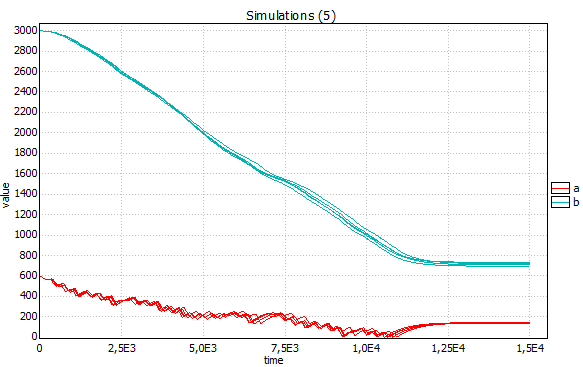
\includegraphics[width=\textwidth]{graphics/simab.png}
	\label{fig:simab}
	\caption{Five simulations of the value of two variables \uppVar{a, b} over time}
\end{figure}

Also it is possible to run probabilities queries, these answers the question; \textit{"What is the probability that some condition will be fulfilled?"}. An example of this can be seen in \cref{fig:pra300}, where we have run the probability that our variable \uppVar{a} will fall below $300$ within time $7200$. \Gls{smc} have then run this by randomly simulating the models behaviour until it with some certainty, within a specified margin of error, knows the chance of the property being true.\\
\Cref{fig:pra300} shows that prior to time $4120$ there are no chance of \uppVar{a} being under $300$, and at time $4520$ it will with certainty be under $300$. For this query it was specified that a $5\%$ uncertainty was acceptable, this resulted in the result seen in \cref{fig:pra300pct} which shows that \gls{smc} was $~90\% - 100\%$ certain \uppVar{a} would fall below $300$. The certainty parameter can be modified to become more precise, at the cost of run time as it will have to run more simulations in order to ensure the correct probability. Using the probability query also allow  for several other types graphs such as probability distribution and frequency histogram.

\begin{figure}[h]
	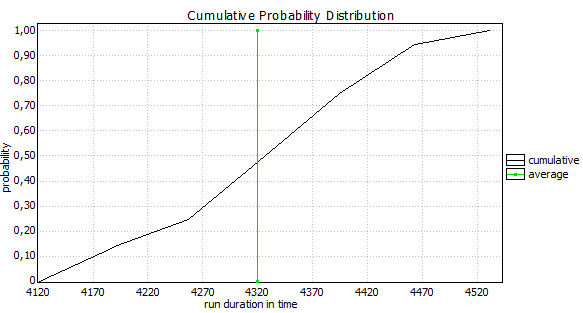
\includegraphics[width=\textwidth]{graphics/pra300.png}
	\label{fig:pra300}
	\caption{Probability over time that the value of (a) will fall under 300}
\end{figure}

\begin{figure}[h]
	\centering
	
\includegraphics[width=8cm]{graphics/pra300pct.png}
	\label{fig:pra300pct}
	\caption{Initial result of running a probability query}
\end{figure}



\section{SMC model} \label{sec:smc_model}
After having produced the best trace from the \gls{cora} model, we get a schedule that contains descriptions of when what payload was executed. These instruction is fed to the \gls{smc} model along the payload description, and relevant information from the described global configurations such as battery settings, schedule length etc.

Since \gls{smc} allows for price with a non-linear rate along with rational numbers, it is possible to implement \gls{kibam}, see \ref{sec:kibam} \nameref{sec:kibam}. The advantage of using the battery model over ideal, implemented in \gls{cora}, is that \gls{kibam} is pessimistic in the sense that \gls{kibam} tends to underestimate the actual battery levels. Because of this \gls{kibam} will be implemented in the \gls{smc} model, instead of the ideal

Our \gls{smc} model consist of four templates plus one instance of a template for each window described in the payload specification. However, it is required that at least one window is defined in the input. This makes a total of 5 plus templates, which are Processor, Insolation, EnergySource, Scheduler, and OrbitWindows(i).\\ 
The \gls{smc} model is based on a UPPAAL implementation of \gls{kibam} \cite{battery_aware_scheduling}, and our \gls{cora} model. The UPPAAL implementation of \gls{kibam} covers scheduling with uncertainty, combined with capturing battery levels during execution of the schedule. \\
The rest of this section we will go over each of the important points in the model, this include the concept of recharging, windows for payloads, payload dependencies ect. 
\ofx{det er ikke blevet beskrevet hvorfor vi laver denne model! ud fra dette ville jeg gætte på det er for KiBaM}

\subsection{Processor}
The initial version of this template was based on a the UPPAAL implementation of \gls{kibam}, which we have then modified to fit our context. The processor template describes the status of the nanosatellites processor, it indicates if it is currently executing a payload, waiting for a payloads deadline to be reached or idling.\\
As the \gls{smc} model receives a schedule from \gls{cora} it does not need to find a payload to execute, instead it will look for the next entry in the array describing what payloads to execute, such an array can be seen in \cref{lst:queue}. This template is responsible for updating the queue, and keeping track of how many payloads have been skipped, and the earnings, in regards to the specified profit.\\
The processor in this model also differs form the one in the \gls{cora} model in the way that in this model, the processor may remain in \uppLoc{Running} for a varying amount of time instead of just the worst execution time for the payload.\\
It synchronises with the scheduler template onthe channel \uppSync{ready!} and then awaits a synchronisation on either \uppSync{run?} or \uppSync{skip?}, while the scheduler determines what to do with the next payload.
\begin{figure}[H]
	\begin{lstlisting}[language=my_c, caption={Payload queue with start times, extracted from the \gls{cora} model}, label=lst:queue, firstnumber=53]
	.
	.
	.
//from cora
int Queue[NumberOfPayloads] = {4, 0, 1, 0, 1, 0, 1, 0, 2, 0, 2, 0, 3, 0, 3, 0};
const int RunStart[NumberOfPayloads] = {0, 50, 100, 140, 190, 230, 280, 320, 370, 410, 460, 500, 550, 590, 640, 680};
	\end{lstlisting}
\end{figure}




\begin{figure}[H]
	\centering
	\begin{tikzpicture}
	%Locations
	\node [init] (l0) [label={[align=left]above:\textcolor{name}{Init}}] {$\cup$};
	\node [location] (l1) [right of=l0, xshift=40mm, label={
		[align=left]above:
		\textcolor{name}{Idle}},
	label={
		[align=center]below:
		\textcolor{invariant}{totalTime <= RunStart[payloadNumber]}
	}] {};
	\node [location] (l2) [right of=l1, xshift=80mm, label={
		[align=left]above:
		\textcolor{name}{Ready}
	}] {};
	\node [location] (l3) [below of=l0, yshift=-40mm, label={
		[align=left]below:
		\textcolor{name}{Done}
	}] {};
	\node [location] (l4) [below of=l1, yshift=-40mm, label={
		[align=left]below:
		\textcolor{name}{Wait}\\
		\textcolor{invariant}{x <= D}
	}] {};
	\node [location] (l5) [below of=l2, yshift=-40mm, label={
		[align=left]below:
		\textcolor{name}{Running}\\
		\textcolor{invariant}{x <= W}
	}] {};
	\path[->,black, thick] (l0) edge node [midway, above][align=left]{
		\textcolor{update}{t=0,i = IIdle,}\\
		\textcolor{update}{setActive()}} (l1);
	\path[->,black, thick] (l1) edge node [midway, above][align=center]{
		\textcolor{guard}{totalTime >=RunStart[payloadNumber]}\\
		\textcolor{sync}{ready!}\\
		\textcolor{update}{x=0, t=0,}\\
		\textcolor{update}{deadline()}} (l2);
	\path[->,black, thick] (l2) edge node [midway, right][align=left]{
		\textcolor{sync}{run?}\\
		\textcolor{update}{x := 0,}\\
		\textcolor{update}{setActive(),}\\
		\textcolor{update}{enqueue()}\\
		\textcolor{update}{earnings +=}\\
		\textcolor{update}{Profit[active]}} (l5);
	\path[->,black, thick] (l2) edge node [midway, left][align=left]{
		\textcolor{sync}{skip?}\\
		\textcolor{update}{payloadNumber ++,}\\
		\textcolor{update}{skipped()}} (l4);
	\path[->,black, thick] (l5) edge node [midway, below][align=left]{
		\textcolor{guard}{x >= B}\\
		\textcolor{update}{dequeue(), active = -1,}\\
		\textcolor{update}{payloadNumber ++}} (l4);
	\path[->,black, thick] (l4) edge node [midway, left][align=left]{
		\textcolor{guard}{x >= D \&\&}\\
		\textcolor{guard}{!done()}\\
		\textcolor{update}{setActive()}} (l1);
	\path[->,black, thick] (l4) edge node [midway, below][align=left]{
		\textcolor{guard}{done()}\\
		\textcolor{update}{on = false,}\\
		\textcolor{update}{active = -1}} (l3);
	\end{tikzpicture}
	\caption{Processor template}
	\label{fig:smc_P}
\end{figure}

\subsection{Scheduler}
When the location \uppLoc{Ready} from Processor is active, two transitions is available to either execute or skip the current payload, each of the transitions are dependent on the scheduler template seen in \cref{fig:smc_S}. This template is responsible for determining if a payload can be run based on all of the restrictions defined, in the payload and environment description, by the user. This includes dependencies, windows, and the battery levels. It checks the windows, dependencies, and the maximum amount of runs per reset, whereas for the battery level it calculates an estimate of what it would be after executing the payload, this is done for both the available, bound and total level.
This is necessary to ensure that a payload does not draw more power than currently available. All of these checks are done on the transition that broadcast \uppSync{run!} indicating that it is safe to execute the payload. \\
If for some reason it is not possible to perform the transition it waits until we either have recharged enough energy or a chance in the windows have occurred, allowing for execution of the payload. If we are not able to perform the payload before the deadline, which is calculated by subtracting worst from the payload deadline, then the other transition is activated leading to a skip of the payload. With dependencies this can have significant consequences to the schedule because the next payload in the schedule may have depended the skipped payload thus resulting in a chain of skipped payloads.

\begin{figure}[H]
	\centering
	\begin{tikzpicture}
	%Locations
	\node [init] (l0) {};
	\node [location] (l1) [right of=l0, xshift=40mm, label={
		[align=left]right:
		\textcolor{invariant}{t <= Payloads[Queue[payloadNumber]][2] - }\\
		\textcolor{invariant}{Payloads[Queue[payloadNumber]][1]}
	}] {};
	\path[->,black, thick] (l1) edge[bend left=50] node [midway, below][align=left]{
		\textcolor{guard}{t == Payloads[Queue[payloadNumber]][2] - }\\
		\textcolor{guard}{Payloads[Queue[payloadNumber]][1]}\\
		\textcolor{sync}{skip!}
	} (l0);
	\path[->,black,thick] (l0) edge node [midway, below][align=left]{
		\textcolor{sync}{ready?}} (l1);
	\path[->,black,thick] (l1) edge[bend right=45] node [midway, above][align=left]{
		\textcolor{guard}{on \&\& mayRun() \&\&}\\
		\textcolor{guard}{0.1 < a * exp(-k2*W)+}\\
		\textcolor{guard}{(((a+b)*k2*c-(Costs[active]+IIdle))*(1.0-exp(-k2*W))}\\
		\textcolor{guard}{-(Costs[active]+IIdle)*c*(k2*W-1.0+exp(-k2*W)))/k2}\\
		\textcolor{guard}{\&\& Threshold < checkB(a,b,totalTime)}\\
		\textcolor{sync}{run!}\\
		\textcolor{update}{runs[active] ++,}\\
		\textcolor{update}{totalRuns[active] ++}
	} (l0);
	\end{tikzpicture}
	\caption{Scheduler template}
	\label{fig:smc_S}
\end{figure}

\subsection{Orbit Windows}
The OrbitWindows template can be found in \cref{fig:smc_OW}, with three locations that each have an in and out going transition creating a loop between them. The overall functionality is similar to the template TaskWindow in the \gls{cora} model. Like in the \gls{cora} model, one instance of OrbitWindows occurs for each defined window. However, in this model it is independent from the rest of the model, in the sense that there are no synchronisations, and is only responsible for keeping track of the window by updating a global variable when a change occur.
%When the first transition, from the initial location, is taken it indicates that the window is now active by changing the global variable \uppVar{inWindow[id]} to 1. When time has passed and window is no longer inside the window the next transition is taken, changing \uppVar{inWindow[id]} to 0. lastly when a full orbit has been performed it resets the clock \uppVar{wtime} with the last transition ending in the initial location.


\subsection{Energy Source} \label{subsec:energy_src}
During the entire schedule we need to keep track of the battery level, as previously mentioned this is done using \gls{kibam}. It is needed to calculate the values of \uppVar{a} and \uppVar{b}, and enable the battery model to recharge\cite{battery_aware_scheduling}. To add the capability of recharging a new location is added to ensure that \uppVar{b} can not exceed its maximum capacity, which is calculated based on the total capacity, so when the model entered the new location it would not add the values of recharge to b. Additionally a guard is set on the transition leading back to \uppLoc{Charging}, that says \uppVar{b} needs to be drained a small amount of power before going back to the initial location. This is done to prevent damaging the battery further. The final template can be found in \cref{fig:smc_ES}.

In \cref{sec:kibam} we described how \gls{kibam} worked as a function of time that calculate the value of a and b at time t, but given we store value a and b and calculate the change to a and b each time tick, more elegant implementation can be constructed\cite{battery_aware_scheduling}. 
\uppVar{a} and \uppVar{b} are represented by clocks and each tick time passes updates the cost on clock \uppVar{a} and \uppVar{b}. This mean that we only need to find the actual increase and decrease that is going to be applied to a and b because we store the value of \uppVar{a} and \uppVar{b}. This is done by the following \gls{smc} invariants presented from the paper and slight modified to work with our restrictions. \uppInv{a' == -i+k*(b/(1-c)-a/c)}, and \uppInv{invariant}{b' == -k*(b/(1-c)-a/c)+(insolation * RechargeRate)}, \uppVar{i} is the current drawn from the battery, which is a combination of \uppVar{IIdle} and \uppVar{Costs[]} depending on where the model is, e.g. if the payload is currently being execute \uppVar{i} will be \uppVar{IIdle} plus \uppVar{Costs[payloadNumber]}. \uppVar{k} determines the flow rate from \uppVar{b} to \uppVar{b}, to check the imbalance between the \uppVar{a} and \uppVar{b} we divide with the ratio of the wells. 

So for example if we have a capacity of $3000$ and a ratio c of $0.2$ this mean that b will be $2400$ and a $600$, in this case if we were to calculate the imbalance like so $(b/(1-c)-a/c)$, this would result in zero because $b/(1-c)$ would be $3000$ and $a/c$ would be $3000$. But lets say a payload had just taken 100 from a in a single tick, the equation would now be $(2400/(1-0.2)-500/0.2)$ resulting in $500$ this would then be multiplied by k to give us the rate of how much from b would need to be added to a. The same is done for b but instead of multiplying by k we multiply by minus k so subtract from b value.
\jfx{skal vi color kode i dette eksempel, jeg syntes ikke det er nødvendigt da det er et eksempel til at vise hvordan udregninger er og ikke har så meget med uppaal at gøre igen.}

Last in the invariant for b is \uppVar{insolation} that is multiplied by \uppVar{RechargeRate}, when we are in an eclipse of the sun \uppVar{insolation} is false result in no recharge being added to \uppVar{b}.


With these changes to the \gls{smc} model we are able to run a schedule with payloads, that have windows and dependencies, with the capability of recharging the battery based on the Insolation tempalte found in \cref{fig:smc_I}, now we only need to consider what queries that should be performed in order to give the most usable data for the users.


%Where the \gls{cora} model finds a trace, the \gls{smc} model will try and rerun the produced trace. This means the \gls{smc} model will execute tasks in the exact same order as the \gls{cora} model.% As this model implements KiBaM it gives a fairly accurate representation of the energy consumption. 

%\Cref{fig:cost_schedule} and \cref{fig:solar_task}, shows the different templates used in the \gls{smc} model. To the left of \cref{fig:cost_schedule} are the energy source. The energy source is responsible for updating the remaining available and bound energy, and in case there are no more available energy, it will synchronise with the scheduler which will then stop running more tasks.
%On the right of \cref{fig:cost_schedule} is the scheduler, it awaits a synchronisation from the tasks in order to ensure that they are ready for execution. The scheduler then estimates if running another task will deplete the battery. If this is the case it will transition back to the initial location preparing to run another task. If running another task would not deplete the battery, the task will be run.

%\begin{figure}[H]%
%	\centering
%	\subfloat
%	{{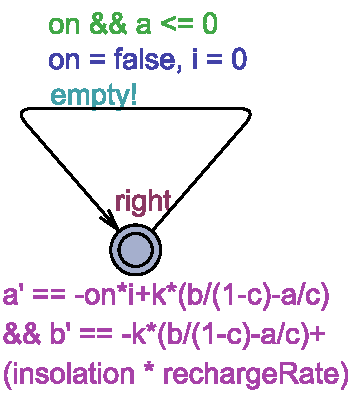
\includegraphics[width=4cm]{graphics/smc_costhandler.pdf} }}%
%	\qquad
%	\subfloat
%	{{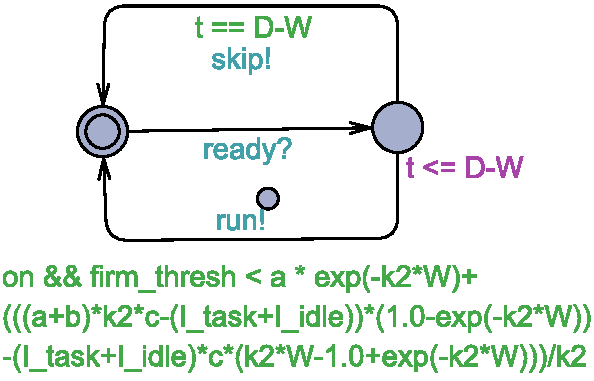
\includegraphics[width=6cm]{graphics/smc_scheduler.pdf} }}%
%	\caption{The \gls{smc} model's energy source(left) and scheduler(right)}%
%	\label{fig:cost_schedule}%
%\end{figure}

%On the left side of \cref{fig:solar_task}, we see the template for the orbit time. It is here assumed that the satellite will spend half its orbit in insolation where it is possible to recharge the battery. It switches the variable \uppVar{Insolation} between true and false, which is used in the calculation of the bound energy.\afx{Kom tilbage hertil når at kibam afsnittet er frdigt. Uddyb om hvordan vores mplementation reflektere teorien fra \cref{sec:kibam}}\\
%The right side of \cref{fig:solar_task} is the template for a task, this indicates that a task can be, ready to be run, running, and inactive. When a task is not running the consumption is lower as indicated by \uppVar{i = I\_idle} which represents the background load of other minor tasks that are not modelled.

%\begin{figure}[H]%
%	\centering
%	\subfloat
%	{{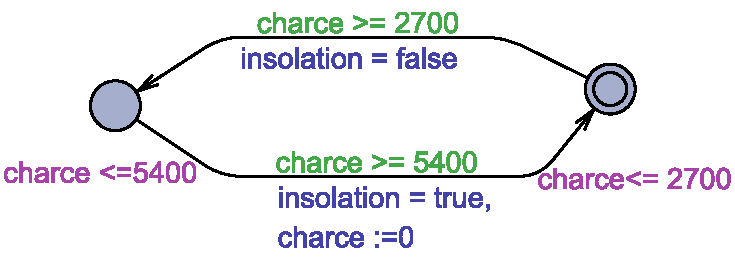
\includegraphics[width=8cm]{graphics/smc_solar.pdf} }}%
%	\qquad
%	\subfloat
%	{{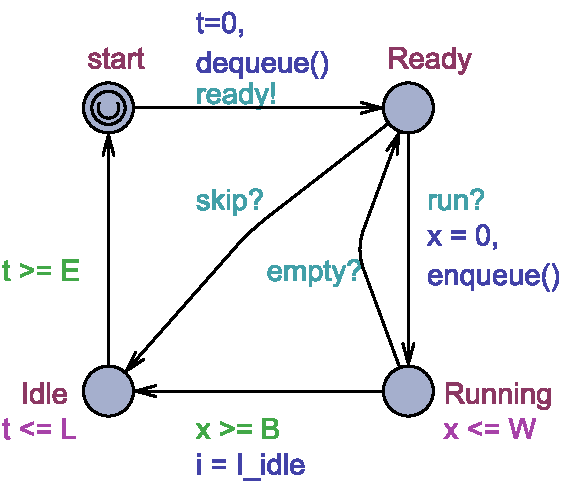
\includegraphics[width=6cm]{graphics/smc_task.pdf} }}%
%	\caption{The \gls{smc} model's representation of solar panels(left) and a task(right)}%
%	\label{fig:solar_task}%
%\end{figure}
%Since the model is made in UPPAAL \gls{smc} we are able to run statistical queries asking for the chance of the available energy falling below some threshold, or to simply track the value of the bound and available energy over time for some specified amount of runs. Examples of such queries can be seen in \cref{eq:pr_low_a_sim_ab}, which indicates, first the chance that the battery level will fall below $55\, \%$ within $43200$ time units. Assuming the time unit is in seconds the example query is for 12 hours. The other query is a simulation of the avilable and bound energy over the same amount of time.\\
%\begin{align}
%Pr[<= 43200] \quad(a <= (c/100)*55)		\nonumber \\
%simulate \quad 1 \quad [<=432000] \quad \{a,b\} 
%\label{eq:pr_low_a_sim_ab}
%\end{align}

%The advantages of running these queries is, that even though the runs in \gls{cora} conclude that a schedule is viable, the probability query may be able to find that running the trace could lead to energy depletion. Also tacking the state of the battery may help to see the effect of the solar panels and the tasks stress on the battery. This is relevant as one or two repetitions of the schedule may not deplete the battery but perhaps ten would, in such case it may be relevant to change some parameters and run it again.
\section{Final Output}\label{sec:final}
The system will output two versions of the schedule and a result file that displays the robustness analysis.
The raw schedule format is produced as a the result from \gls{cora} when we ask it to find the best trace for the chosen schedule duration. The other version of the schedule is one that have been transformed into a Gantt chart for better readability. The robustness analysis results is created by using \gls{smc}'s query feature in order to verify different properties of the schedule and model.

We will not discuss the raw version of the schedule, but a snippet of an example schedule can be found in \myref{appendix:raw_example}.

\input{content/chapter2/gantt_chart.tex}
\input{content/chapter2/queries.tex}
\input{content/chapter2/executing_smc.tex}

\chapter{Evaluation} \label{cha:cha3}

%\input{content/chapter3/...}
\section{Discussion} \label{sec:discussion}

\subsection{Iterative Adjustment of the Nanosatelite Configuration} \label{subsec:disc_itt}
Iterative adjustment of the nanosatelite configuration was never implemented. We decided that we it was not possible to make a correct and non naive implementation within the given time frame of this project. We have decided to include the feature as future work as it we believe it will make the system easier to use.

The downside of having the user to manually adjust their configuration is that they have to decide on which parts of the input that have to be tuned. An automatic process could be able to analyse the schedule for bottlenecks or other parts that would be candidates for change. It can be hard o manually find the variables that may lead to schedule that is not possible, or not robust. They are also limited in what the are able to change, as it is not possible to modify all of the internal variables. Some are hidden anyway to lower the required knowledge of the internal tools, UPPAAL \gls{cora} and \gls{smc}, in order to make the system easier to use. 
%Instead of having to manually adjust the configuration, it could be possible to make the system self configurable at the end of an iteration. Either to explorer new schedules or a more aggressive robustness analysis. For example, \cref{fig:tool_act}  have added an additional step to the tool-chain by allowing the system to loop if the robustness queries were unsatisfied. The system would then have to adjust the variables, such as the [min, max]

Since the iterative adjustment of the nanosatelite configuration have become manual, we have supplied an updated version of the tool-chain which now handles a "No" and "yes" equally in location 6.
\begin{figure}[h]
	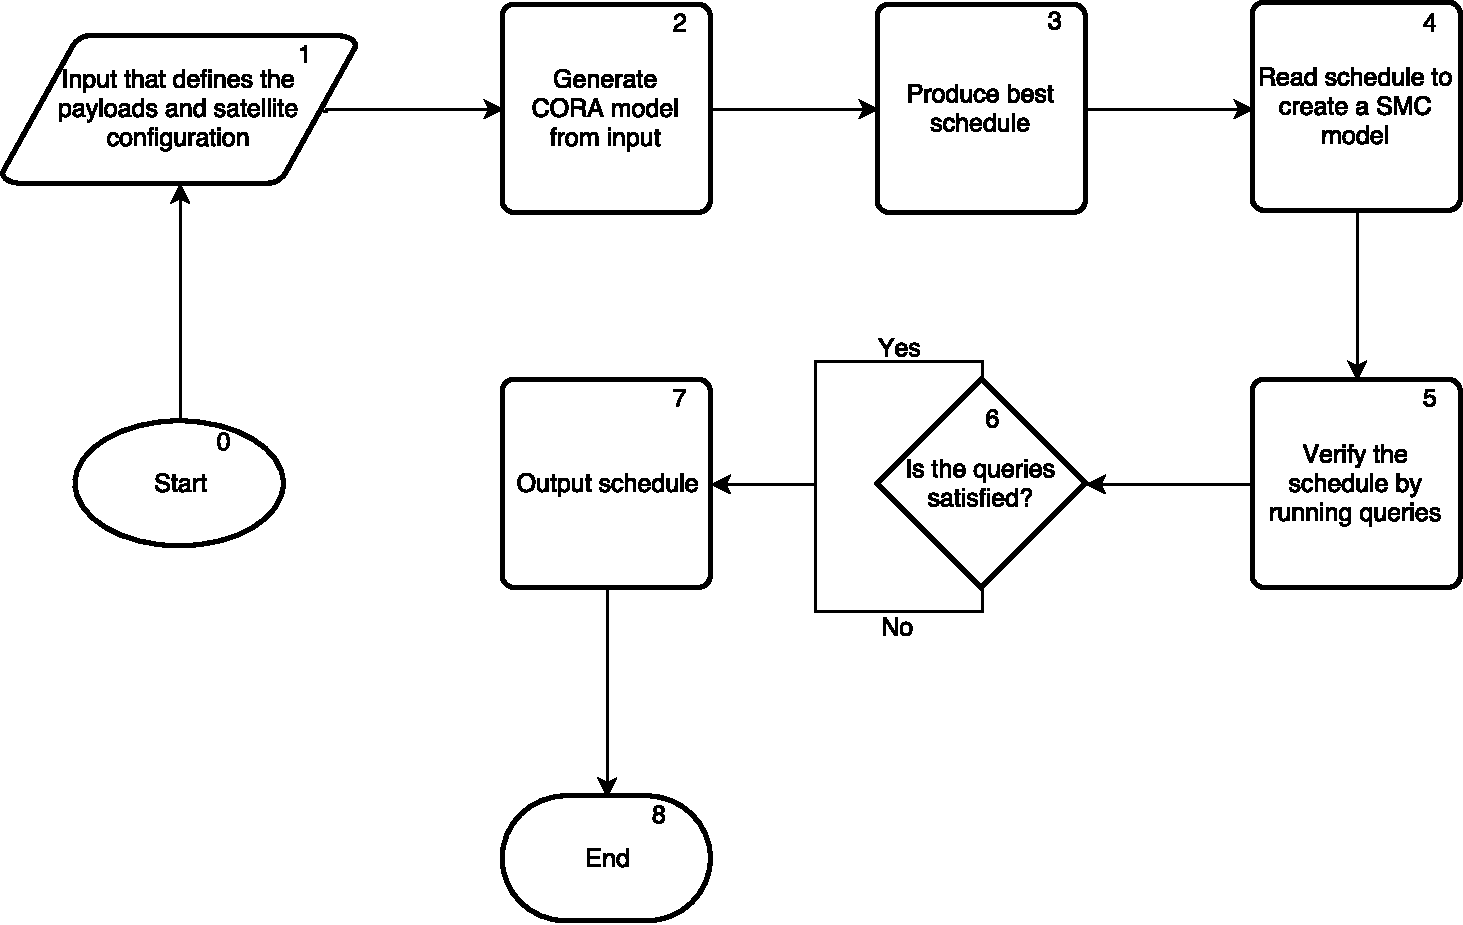
\includegraphics[width=\textwidth]{graphics/flow_act.pdf}
	\caption{Flowchart that displays the actual workflow}
	\label{fig:tool_act}
\end{figure}


\subsection{looping schedules}
problem determine SOC when a battery ends 

logic or in dependencies

\subsection{Battery Lifetime} \label{subsec:disc_life}



\subsection{Proof of viability}
Vi har kun lavet stikproever
Det tilfldige aspekt goer det besvaergeligt (Random search)

\subsection{SMC flaw}
scheduler predict cost of the next payload based on a and b? but dose not take recharge into account or the waiting period of the payload has executed, so potentially it is possible for the battery to go under the threshold if the waiting period after the payload and the next one is enough to have idle energy cost make the battery go under the threshold,  

\subsection{Improving Insolation}
As mentioned in \cref{sec:cora} the model always assume an initial state of insolation, that the nanosatellite is in the sun. Resulting in our schedule only being able to generate schedules for the nanosatellite when it matches our starting point.
This could be corrected by adding new initial location, that have transitions to both of the existing locations, given a variable that will determine which location there should be transitioned to based on the actual position of the satellite.

\chapter{Conclusion} \label{sec:conclusion}
In this chapter we conclude on the report and project as a whole to evaluate the degree of which the problems presented during  \myref{cha:problem} have been fulfilled. This culminated in the following problem statement:

\enquote{How is it possible to produce a schedule that consider multiple requirements, and how is it possible to verify the robustness of such a schedule}

To conclude on the problem statement and to what degree the different requirements have been fulfilled, we must examine and evaluate each of the requirements, and the robustness.

As described in \myref{sec:cora} the \gls{soc} threshold is ensured by the \gls{cora} model, as exceeding this would result in a deadlock, causing the trace to be discarded. Furthermore, in the \gls{smc} model we precalculate the energy consumption to also enforce a payload can only be executed if it will not cause the \gls{soc} to fall below the threshold.  Which these percussions installed, \gls{soc} will always be kept above this threshold.\\
After having completed a payload our \gls{cora} model will immediately start execution of the next payload, if any payload is enabled. However, we do not currently execute payloads as soon as they are enabled if the model is idling, it does not check if a payload is executable until a change in the PaylaodWindow template occurs. Therefore the requirement for payload efficiency is only partially fulfilled.\\
If a payload is defined as only being able to execute in a window, it must never execute at any other time. This is in both models ensured, and the requirement for windows is therefore fulfilled \\
As the schedule is being generated in \gls{cora} with the setting to find the best trace based on the the defined profit, see \myref{sec:cora}, we have archived the goal of maximising profit.\\
Ways of preventing excessive wear on the battery is only considered in our \gls{smc} model enforcing that when the battery reaches maximum capacity, it will stop recharging and not start until a percentage of the capacity has been drained. Given that more could have been done to capture the potential effect of battery wear this is considered partial done. \\
We described wanting to be able to consider, recharge fluctuations, sporadic restarts, and delay to the schedule in \myref{sec:imp_and_add}. However, in the current build it is only possible to check the effects of delaying the schedule, and run some probability queries. This means it is not possible to guarantee the robustness to extend it was desired.

As discussed in \myref{sec:in_and_ass} there are several assumptions and inaccuracies associated with producing our schedule. Despite of us considering several of these to have little to no impact on the schedule, others will most definitely impact it. As this is the case, it will cause a different schedule than what is the actual optimal one. Despite of this we believe our system is still capable of producing a good one.

In conclusion we are able to construct a schedule with the given parameters using \gls{cora}, and partially check its robustness through the \gls{smc} model, which give some indication for the confidence in the produced schedule. This achieve our goal in the main statement. However, evaluating some of the requirements to being partially done we will state that we partially achieve our objectives in generating an optimal schedule and doing some robustness checking on it.
\chapter{Future Work} \label{sec:future}
This chapter covers the ideas we believe is worth pursuing in the future, or was not pursued in this project due to the limited project period.

\subsection*{Memory Considerations}
This topic concerns the physical memory on the nanosatellite in respect to payloads that is producing some amount of data during execution. 
During our meeting with GomSpace, we were introduced to the problem of sending data cost efficiently, as the nanosatellite have multiple windows where it can send data back to Earth. 
But depending on the geographical location, it would cost a fee to use other countries satellite dishes.
It would be interesting to produce schedules that would take this problem into consideration while also balancing power and payload utilisation.
This would make it so that some windows for the data sending payloads are more attractive than others because of their lower fee\cite{gom_space_conversation}.
\paragraph*{Bandwidth}
%Læg op til at man se på båndbredde da det også er en ressource
%    lav tig når vi idler for at gøre dataen mindre
%        komprimering, fjern afstikkere, udregn facit 
Had we implemented the aspect of physical memory, we could also have considered bandwidth. This could be used to determine how long it would take send and receive data to and from Earth. Or instead of having a dependency between sending and collecting data, it would be possible to collect a curtain amount of data till the storage is full and to then send a sub part of the collected data if there is not enough time to send it all.

\subsection*{Start Orbit Time}
When the user is specifying the configuration, it is necessary to specify the start SoC. Something similar for this would be useful for specifying where in the orbit the nanosatellite will start. Currently, we will always start at orbit time zero but this might not reflect the nanosatellites actual position in the orbit.\\
A possible solution would be to allow the user to chose a number within the orbit length, which will be the starting time for the nanosatellite. Alternatively, this number could be an offset for the insolation/eclipse periods and the windows, such the that the start orbit time will still be at zero.

\subsection*{Celestial Bodies Obstructing Line of Sight to the Sun}
The most common celestial body to obstruct the nanosatellite from recharging is the moon with the exception of Earth.
It is questionable how much this would affect the generation of a schedule. If it were to have a real thread, the moon and nanosatellite would need to have close to similar orbital rotation, which is unlikely. We did not believe that this problem could effect schedule's quality, but it made us consider other similar problems.\\
We have made the assumption that the nanosatellite will spent an equal amount of time in insolation and eclipse. This will not always reflect the actual time distribution. We believe that this can be solved by introducing a constant in the configuration. The constant is a percentage that describes the time spent in insolation or eclipse. 

\subsection*{Oval Orbits}
Our models assumes that an orbit is circular so it take equal time the travel a half orbit from any starting point in the orbit. This was not include to simplify the model and deemed unnecessary because the generated schedules only spanning between 12 to 24 hours. 

\subsection*{Payload Dependencies}
Currently a payload can be dependant on the successful execution of another payload. We have introduced dependencies in order to make it possible for the user to help decide the order of the payloads, such that it is only possible to send data after it have been collected.\\
This feature can be improved upon as there is not always a one-to-one relation between the number of times a payload should be executed. In the GomX-3 experience paper\cite{gomx3}, they observed that one L-band payload would require two X-band payloads in order to send all of the data that had been collected. 
Our models does not directly allow for such a relation as the completion of the dependency unlocks the execution of the dependant payload until a function locks it again. Currently, the locking function is only called when all payloads are no longer allowed to be executed because they have hit their maximum of allowed executions. 
This is what we are referring to when we state that it is possible to indirectly make this relationship, as the maximum allowed executions can be set to the same amount as the dependant payload requires it to execute. By this approch it can be defined that \textit{L} may be run once, and \textit{X} is dependant on \textit{L} and may be run twice.\\
This however is more of a workaround and we believe that an actually implementation of these dependencies would increase the expressiveness of the payload descriptions

\subsection*{Satellite Attitude \& Drag}
The attitude of the nanosatellite is not modelled, which results in the schedule not being as payload efficient as it could have been if we did consider the attitude. Bisgaard et al. 2016\cite{gomx3} declared that the X and L-band equipment is installed on opposite surfaces of the GomX-3 nanosatellite, which mean that only of them may be used at the time, as they have to be pointed towards Earth. They accommodated this by implementing logic in their model for slewing the nanosatellite into place before the payload was executed. Our approach is to advice the user into including the possible time it takes to slew the satellite before a payload is executed. This has the effect that the worst case execution time of the payloads that are attitude dependent, is increased by that of time it takes to slew into place. Another effect is that the tool may produce a schedule were the nanosatellite has to slew back and forth multiple times in a row, instead of bundling payloads that needs the same orientation.\\
Support for setting the nanosatellite's attitude, and specifying the dependence of it on payloads would solve this inefficiency.
The positive effect of not considering this aspect is the reduced state space in the \gls{cora} model. However, We do believe that it is worth testing how a schedule may be produced differently, if the feature were to be implemented.
%Our tool have no notion of satellite attitude, this is intentionally left out, because a payloads execution is defined by the user and could just include the time it takes to slew the nanosatellite in the payload description. By doing it this way we reduce the number of possible schedules that can exist. Some complications arise when going this direction, if slew is calculated in a payload that mean if another payload needs to face the same angle it also needs to add the time required to slew the nanosatellite. which is wasteful because they would be able to save time if the could slew and perform two payloads and then resume its original orientation.


\subsection*{Battery Wear}
Battery deteriorating is not supported in our solution, but since the user can theoretically calculate the actual capacity of the battery and set the maximum capacity to that value, it is possible to pass the information to the model. Furthermore, the scheduler is not trying to minimise battery wear when producing a schedule. However, a location have been added to the \gls{smc} model in order to avoid overcharging the battery, as explained in \myref{sec:smc_model}.\\
Wognsen et al. 2015\cite{score_function} expresses how it is important to find a balance between not wearing the battery and doing something worthwhile with the nanosatellite i.e. executing payloads. We believe that since our tool has an emphasis on battery usage, the ability to model battery wear and avoid schedules that have a high impact on it, will be sensible to implement. 

\subsection*{Restarts}
In \myref{sec:imp_and_add} we described a desire for incorporating unpredictable restarts into the schedule, in order to test the schedules robustness. However, this was never implemented. Implementing this could have been done in several ways e.g. restarts could have been added to the schedule at random when generating the \gls{smc} model, or a septate template could have been added to the \gls{smc} model, which would cause the processor and scheduler templates to leave their current location for a duration of time.

\subsection*{Starting Values} \label{ssec:start_val}
In \myref{sec:in_and_ass} we discussed that, despite of the many input parameters fed to the system, we believe it could have been beneficial to include more in order to better represent the nanosatellites current state. Specificity we believe a representation of current amount of executions per payload should have been included. This is important as the last generated schedule may have ended with several payloads having been executed, potentially fulfilling some dependencies, meaning other payloads should be executable from the beginning of the new schedule.

\subsection*{Multiple Windows per Payload}\label{ssec:multi_window}
As described in \myref{sec:in_and_ass}, there are multiple stations on Earth with which the nanosatellite can communicate it would be a beneficial addition to allow a payload to be associated with multiple windows. As this is not currently included it may have a significant impact on the generated schedule, since the satellite may be ready to transmit data to Earth at time 20 but is only defined to have a window at time 70-80 despite of it, in reality, also having one at time 30-40. This could be included by making an update to the script feeding the payload description to the models.




%%Indsæt rapportens filer her!!%%

%%Glossary
\printglossary[style=long]

%% List of figures
\listoffigures

%% list of tables
\listoftables

%% List of listings
\lstlistoflistings

%% List of Fx notes
%\newpage
%\listoffixmes

%%%% Kilder %%%%
\begingroup
	\raggedright
%    \bibliography{bib}											% Litteraturlisten inkluderes
\printbibliography
\endgroup
%%%% Appendiks %%%%
\appendix														% Appendiks/bilag start - giver chapter bogstaver i stedet for tal
\clearforchapter												% Sikrer at pagestylen aktiveres paa den rigtige side
\phantomsection													% Kunstigt afsnit, som hyperlinks kan 'holde fast i'
\pdfbookmark[0]{Appendices}{appendices}							% Tildeler en klikbar bookmark til den endelige PDF

\chapter{Variable Loads}\label{cp:VL}
\begin{table}[]
\centering
\begin{tabular}{|l|l|}
\hline
Cases & Timing, min \\ \hline
\rowcolor[HTML]{EFEFEF} 
\#1 & (0, 19.5, 26.0) \\ \hline
\#2 & (0, 31.0, 41.3) \\ \hline
\rowcolor[HTML]{EFEFEF} 
\#3 & (0, 41.0, 54.6) \\ \hline
\#4 & (0, 74.6, 99.5) \\ \hline
\rowcolor[HTML]{EFEFEF} 
\#5 & (0, 105.7, 140.9) \\ \hline
\#6 & (0, 19.5, 29.9) \\ \hline
\rowcolor[HTML]{EFEFEF} 
\#7 & (0, 19.5, 22.1) \\ \hline
\#8 & (0, 23.4, 29.9) \\ \hline
\rowcolor[HTML]{EFEFEF} 
\#9 & (0, 15.6, 22.1) \\ \hline
\#10 & (0, 0.5, 5.5, 10.5, 35.5, 60.5, 85.5, 110.5) \\ \hline
\end{tabular}
\label{table:variable_loads_list}
\caption{Data taken from \cite{battery_model}}
\end{table}
\chapter{\gls{smc} models}\label{cp:smc_models}
\section{Processor}
\begin{figure}[H]
	\centering
	\begin{tikzpicture}
	%Locations
	\node [init] (l0) {$\cup$};
	\node [location] (l1) [right of=l0, xshift=40mm, label={
		[align=left]above:
		\textcolor{name}{PrepNext}},
	label={
		[align=center]below:
		\textcolor{invariant}{totalTime <= RunStart[payloadNumber]}
	}] {};
	\node [location] (l2) [right of=l1, xshift=80mm, label={
		[align=left]above:
		\textcolor{name}{Ready}
	}] {};
	\node [location] (l3) [below of=l0, yshift=-40mm, label={
		[align=left]below:
		\textcolor{name}{Done}
	}] {};
	\node [location] (l4) [below of=l1, yshift=-40mm, label={
		[align=left]below:
		\textcolor{name}{Idle}\\
		\textcolor{invariant}{x <= D}
	}] {};
	\node [location] (l5) [below of=l2, yshift=-40mm, label={
		[align=left]below:
		\textcolor{name}{Running}\\
		\textcolor{invariant}{x <= W}
	}] {};
	\path[->,black] (l0) edge node [midway, above][align=left]{
		\textcolor{update}{t=0,i = IIdle,}\\
		\textcolor{update}{setActive()}} (l1);
	\path[->,black] (l1) edge node [midway, above][align=center]{
		\textcolor{guard}{totalTime >=RunStart[payloadNumber]}\\
		\textcolor{sync}{ready!}\\
		\textcolor{update}{x=0, t=0,}\\
		\textcolor{update}{dequeue()}} (l2);
	\path[->,black] (l2) edge node [midway, left][align=left]{
		\textcolor{sync}{run?}\\
		\textcolor{update}{x := 0,}\\
		\textcolor{update}{setActive(),}\\
		\textcolor{update}{enqueue()}} (l5);
	\path[->,black] (l5) edge[bend right=45] node [midway, right][align=left]{
		\textcolor{sync}{empty?}} (l2);
	\path[->,black] (l4) edge node [midway, left][align=left]{
		\textcolor{sync}{skip?}\\
		\textcolor{update}{payloadNumber ++,}\\
		\textcolor{update}{skipped()}} (l2);
	\path[->,black] (l5) edge node [midway, below][align=left]{
		\textcolor{guard}{x >= B}\\
		\textcolor{update}{i = IIdle, active = -1,}\\
		\textcolor{update}{payloadNumber ++}} (l4);
	\path[->,black] (l4) edge node [midway, left][align=left]{
		\textcolor{guard}{x >= D \&\&}\\
		\textcolor{guard}{!done()}\\
		\textcolor{update}{setActive()}} (l1);
	\path[->,black] (l4) edge node [midway, below][align=left]{
		\textcolor{guard}{done()}\\
		\textcolor{update}{on = false,}\\
		\textcolor{update}{active = -1}} (l3);
	\end{tikzpicture}
	\caption{Processor template}
	\label{fig:smc_P}
\end{figure}

\section{Insolation}
\begin{figure}[H]
	\centering
	\begin{tikzpicture}
	%Locations
	\node [init] (l0) [label={
		[align=left]left:
		\textcolor{invariant}{charge<= OrbitTime/2}
	}] {};
	\node [location] (l1) [right of=l0, xshift=40mm, label={
		[align=left]right:
		\textcolor{invariant}{charge <=OrbitTime}
	}] {};
	\path[->,black] (l0) edge[bend left=45] node [midway, above][align=left]{
		\textcolor{guard}{charge >= OrbitTime/2}\\
		\textcolor{update}{insolation = false}} (l1);
	\path[->,black] (l1) edge[bend left=45] node [midway, below][align=left]{
		\textcolor{guard}{charge >= OrbitTime}\\
		\textcolor{update}{insolation = true,}\\
		\textcolor{update}{charge :=0}} (l0);
	\end{tikzpicture}
	\caption{Insolation template}
	\label{fig:smc_I}
\end{figure}

\section{EnergySource}
\begin{figure}[H]
	\centering
	\begin{tikzpicture}
	%Locations
	\node [init] (l0) [label={
		[align=left]left:
		\textcolor{invariant}{a' == -on*i+k*(b/(1-c)-a/c)}\\
		\textcolor{invariant}{\&\& b' == -k*(b/(1-c)-a/c)}\\
		\textcolor{invariant}{+(insolation * RechargeRate)}
	}] {};
	\node [location] (l1) [right of=l0, xshift=40mm, label={
		[align=left]right:
		\textcolor{invariant}{a' == -on*i+k*(b/(1-c)-a/c)}\\
		\textcolor{invariant}{\&\& b' == -k*(b/(1-c)-a/c)}
	}] {};
	\path[->,black] (l0) edge node [midway, above][align=left]{
		\textcolor{guard}{b > MaxB}\\
		\textcolor{sync}{capacityFull!}} (l1);
	\path[->,black] (l1) edge[bend left=45] node [midway, below][align=left]{
		\textcolor{guard}{b < c\_C}\\
		\textcolor{sync}{capacityFull!}} (l0);
	\path[->,black] (l1) edge[loop above] node [midway, above][align=left]{
		\textcolor{guard}{on \&\& a <= 0}\\
		\textcolor{sync}{empty!}\\
		\textcolor{update}{on = false, i = 0}} (l1);
	\path[->,black] (l0) edge[loop above] node [midway, above][align=left]{
		\textcolor{guard}{on \&\& a <= 0}\\
		\textcolor{sync}{empty!}\\
		\textcolor{update}{on = false, i = 0}} (l0);
	\end{tikzpicture}
	\caption{EnergySource template}
	\label{fig:smc_ES}
\end{figure}

\section{Scheduler}
\begin{figure}[H]
	\centering
	\begin{tikzpicture}
	%Locations
	\node [init] (l0) {};
	\node [location] (l1) [right of=l0, xshift=40mm, label={
		[align=left]right:
		\textcolor{invariant}{t <= Payloads[Queue[payloadNumber]][2] - }\\
		\textcolor{invariant}{Payloads[Queue[payloadNumber]][1]}
	}] {};
	\path[->,black] (l1) edge[bend left=50] node [midway, below][align=left]{
		\textcolor{guard}{t == Payloads[Queue[payloadNumber]][2] - }\\
		\textcolor{guard}{Payloads[Queue[payloadNumber]][1]}\\
		\textcolor{sync}{skip!}
	} (l0);
	\path[->,black] (l0) edge node [midway, below][align=left]{
		\textcolor{sync}{ready?}} (l1);
	\path[->,black] (l1) edge[bend right=45] node [midway, above][align=left]{
		\textcolor{guard}{on \&\& mayRun() \&\&}\\
		\textcolor{guard}{FirmThreshold < a * exp(-k2*W)+}\\
		\textcolor{guard}{(((a+b)*k2*c-(IPayload+IIdle))*(1.0-exp(-k2*W))}\\
		\textcolor{guard}{-(IPayload+IIdle)*c*(k2*W-1.0+exp(-k2*W)))/k2}\\
		\textcolor{sync}{run!}\\
		\textcolor{update}{runs[active] ++,}\\
		\textcolor{update}{totalRuns[active] ++}
	} (l0);
	\end{tikzpicture}
	\caption{Task template}
	\label{fig:smc_S}
\end{figure}

\section{OrbitWindows}
\begin{figure}[H]
	\centering
	\begin{tikzpicture}
	%Locations
	\node [init] (l0) [label={
		[align=left]left:
		\textcolor{invariant}{wtime <= Window[id][0]}}] {};
	\node [location] (l1) [right of=l0, xshift=40mm, label={
		[align=left]right:
		\textcolor{invariant}{wtime <= Window[id][1]}
	}] {};
	\node [location] (l2) [below of=l0, xshift=25mm, yshift=-40mm, label={
		[align=left]below:
		\textcolor{invariant}{wtime <= OrbitTime}
	}] {};
	\path[->,black] (l0) edge node [midway, above][align=left]{
		\textcolor{guard}{wtime >= Window[id][0]}\\
		\textcolor{update}{setRunnable(),}\\
		\textcolor{update}{inWindow[id] = 1}
	} (l1);
	\path[->,black] (l1) edge node [midway, right][align=left]{
		\textcolor{guard}{wtime >= Window[id][1]}\\
		\textcolor{update}{setRunnable(),}\\
		\textcolor{update}{inWindow[id] = 0}
	} (l2);
	\path[->,black] (l2) edge node [midway, left][align=left]{
		\textcolor{guard}{wtime >= OrbitTime}\\
		\textcolor{update}{wtime = 0}
	} (l0);
	\end{tikzpicture}
	\caption{OrbitWindows template}
	\label{fig:smc_OW}
\end{figure}

\chapter{Raw Schedule Example}\label{appendix:raw_example}
\begin{figure}[H]
	\begin{lstlisting}[caption={The raw schedule format. Note the first transition at line 5 that indicate we enter a running state i.e. we start executing a payload. We stop executing the payload after 15 time units(minutes) have passed.}, label=lst:raw, language=text]
	State:
	( Processor.Ready Scheduler._id7 Insolation._id10 PayloadWindow(0)._id14 PayloadWindow(1).In )
	ins=50 t_time=2120 Processor.x=20 Insolation.splitTime=6 PayloadWindow(0).wtime=50 PayloadWindow(1).wtime=50 on=1 batteryCap=3516 active=0 runs[0]=2 runs[1]=3 runs[2]=0 runs[3]=0 runs[4]=1 tRuns[0]=11 tRuns[1]=12 tRuns[2]=6 tRuns[3]=6 tRuns[4]=4 available[0]=1 available[1]=0 available[2]=0 available[3]=0 available[4]=1 runnable[0]=1 runnable[1]=0 runnable[2]=0 runnable[3]=0 runnable[4]=0 Processor.queue[0]=-1 Processor.queue[1]=-1 Processor.queue[2]=-1 Processor.queue[3]=-1 Processor.queue[4]=-1 Processor.runCost=2 Scheduler.threshold=1 Insolation.chargeCount=0 rate=1 cost=7890
	
	Transitions:
	Scheduler._id7->Scheduler._id8 { 1, run!, 1 }
	Processor.Ready->Processor.Running { runnable[active] == 1 && !checkBattery(), run?, updateBattery(), calcCost() }
	
	State:
	( Processor.Running Scheduler._id8 Insolation._id10 PayloadWindow(0)._id14 PayloadWindow(1).In )
	ins=50 t_time=2120 Processor.x=0 Insolation.splitTime=6 PayloadWindow(0).wtime=50 PayloadWindow(1).wtime=50 on=1 batteryCap=3468 active=0 runs[0]=3 runs[1]=3 runs[2]=0 runs[3]=0 runs[4]=1 tRuns[0]=12 tRuns[1]=12 tRuns[2]=6 tRuns[3]=6 tRuns[4]=4 available[0]=1 available[1]=0 available[2]=0 available[3]=0 available[4]=1 runnable[0]=1 runnable[1]=0 runnable[2]=0 runnable[3]=0 runnable[4]=0 Processor.queue[0]=-1 Processor.queue[1]=-1 Processor.queue[2]=-1 Processor.queue[3]=-1 Processor.queue[4]=-1 Processor.runCost=2 Scheduler.threshold=1 Insolation.chargeCount=0 rate=2 cost=7890
	
	Delay: 15
	
	State:
	( Processor.Running Scheduler._id8 Insolation._id10 PayloadWindow(0)._id14 PayloadWindow(1).In )
	ins=65 t_time=2135 Processor.x=15 Insolation.splitTime=21 PayloadWindow(0).wtime=65 PayloadWindow(1).wtime=65 on=1 batteryCap=3468 active=0 runs[0]=3 runs[1]=3 runs[2]=0 runs[3]=0 runs[4]=1 tRuns[0]=12 tRuns[1]=12 tRuns[2]=6 tRuns[3]=6 tRuns[4]=4 available[0]=1 available[1]=0 available[2]=0 available[3]=0 available[4]=1 runnable[0]=1 runnable[1]=0 runnable[2]=0 runnable[3]=0 runnable[4]=0 Processor.queue[0]=-1 Processor.queue[1]=-1 Processor.queue[2]=-1 Processor.queue[3]=-1 Processor.queue[4]=-1 Processor.runCost=2 Scheduler.threshold=1 Insolation.chargeCount=0 rate=2 cost=7920
	
	Transitions:
	Processor.Running->Processor.Wait { x >= TaskTimes[active][1], tau, 1 }
	\end{lstlisting}
\end{figure}



\end{document}
